% Options for packages loaded elsewhere
\PassOptionsToPackage{unicode}{hyperref}
\PassOptionsToPackage{hyphens}{url}
\PassOptionsToPackage{dvipsnames,svgnames,x11names}{xcolor}
%
\documentclass[
  11pt,
  a4paper,
]{article}

\usepackage{amsmath,amssymb}
\usepackage{setspace}
\usepackage{iftex}
\ifPDFTeX
  \usepackage[T1]{fontenc}
  \usepackage[utf8]{inputenc}
  \usepackage{textcomp} % provide euro and other symbols
\else % if luatex or xetex
  \usepackage{unicode-math}
  \defaultfontfeatures{Scale=MatchLowercase}
  \defaultfontfeatures[\rmfamily]{Ligatures=TeX,Scale=1}
\fi
\usepackage{lmodern}
\ifPDFTeX\else  
    % xetex/luatex font selection
\fi
% Use upquote if available, for straight quotes in verbatim environments
\IfFileExists{upquote.sty}{\usepackage{upquote}}{}
\IfFileExists{microtype.sty}{% use microtype if available
  \usepackage[]{microtype}
  \UseMicrotypeSet[protrusion]{basicmath} % disable protrusion for tt fonts
}{}
\makeatletter
\@ifundefined{KOMAClassName}{% if non-KOMA class
  \IfFileExists{parskip.sty}{%
    \usepackage{parskip}
  }{% else
    \setlength{\parindent}{0pt}
    \setlength{\parskip}{6pt plus 2pt minus 1pt}}
}{% if KOMA class
  \KOMAoptions{parskip=half}}
\makeatother
\usepackage{xcolor}
\usepackage[top=2.4cm,bottom=2.4cm,left=2.5cm,right=2.5cm]{geometry}
\setlength{\emergencystretch}{3em} % prevent overfull lines
\setcounter{secnumdepth}{2}


\providecommand{\tightlist}{%
  \setlength{\itemsep}{0pt}\setlength{\parskip}{0pt}}\usepackage{longtable,booktabs,array}
\usepackage{calc} % for calculating minipage widths
% Correct order of tables after \paragraph or \subparagraph
\usepackage{etoolbox}
\makeatletter
\patchcmd\longtable{\par}{\if@noskipsec\mbox{}\fi\par}{}{}
\makeatother
% Allow footnotes in longtable head/foot
\IfFileExists{footnotehyper.sty}{\usepackage{footnotehyper}}{\usepackage{footnote}}
\makesavenoteenv{longtable}
\usepackage{graphicx}
\makeatletter
\def\maxwidth{\ifdim\Gin@nat@width>\linewidth\linewidth\else\Gin@nat@width\fi}
\def\maxheight{\ifdim\Gin@nat@height>\textheight\textheight\else\Gin@nat@height\fi}
\makeatother
% Scale images if necessary, so that they will not overflow the page
% margins by default, and it is still possible to overwrite the defaults
% using explicit options in \includegraphics[width, height, ...]{}
\setkeys{Gin}{width=\maxwidth,height=\maxheight,keepaspectratio}
% Set default figure placement to htbp
\makeatletter
\def\fps@figure{htbp}
\makeatother

\usepackage{booktabs}
\usepackage{longtable}
\usepackage{array}
\usepackage{multirow}
\usepackage{wrapfig}
\usepackage{float}
\usepackage{colortbl}
\usepackage{pdflscape}
\usepackage{tabu}
\usepackage{threeparttable}
\usepackage{threeparttablex}
\usepackage[normalem]{ulem}
\usepackage{makecell}
\usepackage{xcolor}
\makeatletter
\@ifpackageloaded{caption}{}{\usepackage{caption}}
\AtBeginDocument{%
\ifdefined\contentsname
  \renewcommand*\contentsname{Table of contents}
\else
  \newcommand\contentsname{Table of contents}
\fi
\ifdefined\listfigurename
  \renewcommand*\listfigurename{List of Figures}
\else
  \newcommand\listfigurename{List of Figures}
\fi
\ifdefined\listtablename
  \renewcommand*\listtablename{List of Tables}
\else
  \newcommand\listtablename{List of Tables}
\fi
\ifdefined\figurename
  \renewcommand*\figurename{Figure}
\else
  \newcommand\figurename{Figure}
\fi
\ifdefined\tablename
  \renewcommand*\tablename{Table}
\else
  \newcommand\tablename{Table}
\fi
}
\@ifpackageloaded{float}{}{\usepackage{float}}
\floatstyle{ruled}
\@ifundefined{c@chapter}{\newfloat{codelisting}{h}{lop}}{\newfloat{codelisting}{h}{lop}[chapter]}
\floatname{codelisting}{Listing}
\newcommand*\listoflistings{\listof{codelisting}{List of Listings}}
\makeatother
\makeatletter
\makeatother
\makeatletter
\@ifpackageloaded{caption}{}{\usepackage{caption}}
\@ifpackageloaded{subcaption}{}{\usepackage{subcaption}}
\makeatother
\ifLuaTeX
  \usepackage{selnolig}  % disable illegal ligatures
\fi
\usepackage[style=authoryear-comp,]{biblatex}
\addbibresource{references.bib}
\usepackage{bookmark}

\IfFileExists{xurl.sty}{\usepackage{xurl}}{} % add URL line breaks if available
\urlstyle{same} % disable monospaced font for URLs
\hypersetup{
  pdftitle={Forecast Reconciliation for Land Transfer Duty},
  pdfauthor={Hoang Do},
  colorlinks=true,
  linkcolor={blue},
  filecolor={Maroon},
  citecolor={Blue},
  urlcolor={Blue},
  pdfcreator={LaTeX via pandoc}}

%% CAPTIONS
\usepackage{caption}
\DeclareCaptionStyle{italic}[justification=centering]
 {labelfont={bf},textfont={it},labelsep=colon}
\captionsetup[figure]{style=italic,format=hang,singlelinecheck=true}
\captionsetup[table]{style=italic,format=hang,singlelinecheck=true}

%% FONT
\usepackage{bera}
\usepackage[charter]{mathdesign}
\usepackage[scale=0.9]{sourcecodepro}
\usepackage[lf,t]{FiraSans}
\usepackage{fontawesome}

%% HEADERS AND FOOTERS
\usepackage{fancyhdr}
\pagestyle{fancy}
\rfoot{\Large\sffamily\raisebox{-0.1cm}{\textbf{\thepage}}}
\makeatletter
\lhead{\textsf{\expandafter{\@title}}}
\makeatother
\rhead{}
\cfoot{}
\setlength{\headheight}{15pt}
\renewcommand{\headrulewidth}{0.4pt}
\renewcommand{\footrulewidth}{0.4pt}
\fancypagestyle{plain}{%
\fancyhf{} % clear all header and footer fields
\fancyfoot[C]{\sffamily\thepage} % except the center
\renewcommand{\headrulewidth}{0pt}
\renewcommand{\footrulewidth}{0pt}}

%% MATHS
\usepackage{bm,amsmath}
\allowdisplaybreaks

%% GRAPHICS
\makeatletter
\def\fps@figure{htbp}
\makeatother
\setcounter{topnumber}{2}
\setcounter{bottomnumber}{2}
\setcounter{totalnumber}{4}
\renewcommand{\topfraction}{0.85}
\renewcommand{\bottomfraction}{0.85}
\renewcommand{\textfraction}{0.15}
\renewcommand{\floatpagefraction}{0.8}

%% SECTION TITLES
\usepackage[compact,sf,bf]{titlesec}
\titleformat*{\section}{\Large\sf\bfseries\color[rgb]{0.7,0,0}}
\titleformat*{\subsection}{\large\sf\bfseries\color[rgb]{0.7,0,0}}
\titleformat*{\subsubsection}{\sf\bfseries\color[rgb]{0.7,0,0}}
\titlespacing{\section}{0pt}{2ex}{.5ex}
\titlespacing{\subsection}{0pt}{1.5ex}{0ex}
\titlespacing{\subsubsection}{0pt}{.5ex}{0ex}


%% BIBLIOGRAPHY.

\makeatletter
\@ifpackageloaded{biblatex}{
\ExecuteBibliographyOptions{bibencoding=utf8,minnames=1,maxnames=3, maxbibnames=99,dashed=false,terseinits=true,giveninits=true,uniquename=false,uniquelist=false,doi=false, isbn=false,url=true,sortcites=false}
\DeclareFieldFormat{url}{\texttt{\url{#1}}}
\DeclareFieldFormat[article]{pages}{#1}
\DeclareFieldFormat[inproceedings]{pages}{\lowercase{pp.}#1}
\DeclareFieldFormat[incollection]{pages}{\lowercase{pp.}#1}
\DeclareFieldFormat[article]{volume}{\mkbibbold{#1}}
\DeclareFieldFormat[article]{number}{\mkbibparens{#1}}
\DeclareFieldFormat[article]{title}{\MakeCapital{#1}}
\DeclareFieldFormat[article]{url}{}
\DeclareFieldFormat[inproceedings]{title}{#1}
\DeclareFieldFormat{shorthandwidth}{#1}
\usepackage{xpatch}
\xpatchbibmacro{volume+number+eid}{\setunit*{\adddot}}{}{}{}
% Remove In: for an article.
\renewbibmacro{in:}{%
  \ifentrytype{article}{}{%
  \printtext{\bibstring{in}\intitlepunct}}}
\AtEveryBibitem{\clearfield{month}}
\AtEveryCitekey{\clearfield{month}}
\DeclareDelimFormat[cbx@textcite]{nameyeardelim}{\addspace}
\renewcommand*{\finalnamedelim}{\addspace\&\space}
}{}
\makeatother

%% PAGE BREAKING to avoid widows and orphans
\clubpenalty = 2000
\widowpenalty = 2000
\usepackage{microtype}% Placement of logos

\RequirePackage[absolute,overlay]{textpos}
\setlength{\TPHorizModule}{1cm}
\setlength{\TPVertModule}{1cm}
\def\placefig#1#2#3#4{\begin{textblock}{.1}(#1,#2)\rlap{\includegraphics[#3]{#4}}\end{textblock}}

% Title and date

\title{Forecast Reconciliation for Land Transfer Duty}
\date{1 August 2024}

\def\Date{\number\day}
\def\Month{\ifcase\month\or
 January\or February\or March\or April\or May\or June\or
 July\or August\or September\or October\or November\or December\fi}
\def\Year{\number\year}

%%%% PAGE STYLE FOR FRONT PAGE OF REPORTS

\makeatletter
\def\organization#1{\gdef\@organization{#1}}
\def\telephone#1{\gdef\@telephone{#1}}
\def\email#1{\gdef\@email{#1}}
\makeatother
  \organization{The Department of Treasury and Finance}

  \def\name{Department of\newline Econometrics \&\newline Business Statistics}

  \telephone{(03) 9903 4416}

  \email{vdoo0002@student.monash.edu}

\def\webaddress{\url{https://www.monash.edu/business/ebs}}
\def\abn{12 377 614 012}
\def\extraspace{\vspace*{1.6cm}}
\makeatletter
\def\contactdetails{\faicon{phone} & \@telephone \\
                    \faicon{envelope} & \@email}
\makeatother

\usepackage[absolute,overlay]{textpos}
\setlength{\TPHorizModule}{1cm}
\setlength{\TPVertModule}{1cm}

%%%% FRONT PAGE OF REPORTS

\def\reporttype{Report for}

\long\def\front#1#2#3{
\newpage
\begin{textblock}{7}(12.7,28.2)\hfill

\includegraphics[height=0.6cm]{AACSB}~~~

\includegraphics[height=0.6cm]{EQUIS}~~~

\includegraphics[height=0.6cm]{AMBA}
\end{textblock}
\begin{singlespacing}
\thispagestyle{empty}
\vspace*{-1.4cm}
\hspace*{-1.4cm}
\hbox to 16cm{
  \hbox to 6.5cm{\vbox to 14cm{\vbox to 25cm{
    
\includegraphics[width=6cm]{monash2}
    \vfill
    
\includegraphics[width=2cm]{MBSportrait}
    \vspace{0.4cm}
    \par
    \parbox{6.3cm}{\raggedright
      \sf\color[rgb]{0.00,0.00,0.70}
      {\large\textbf{\name}}\par
      \vspace{.7cm}
      \tabcolsep=0.12cm\sf\small
      \begin{tabular}{@{}ll@{}}\contactdetails
      \end{tabular}
      \vspace*{0.3cm}\par
      ABN: \abn\par
    }
  }\vss}\hss}
  \hspace*{0.2cm}
  \hbox to 1cm{\vbox to 14cm{\rule{1pt}{26.8cm}\vss}\hss\hfill}
  \hbox to 10cm{\vbox to 14cm{\vbox to 25cm{
      \vspace*{3cm}\sf\raggedright
      \parbox{10cm}{\sf\raggedright\baselineskip=1.2cm
         \fontsize{24.88}{30}\color[rgb]{0.70,0.00,0.00}\sf\textbf{#1}}
      \par
      \vfill
      \large
      \vbox{\parskip=0.8cm #2}\par
      \vspace*{2cm}\par
      \reporttype\\[0.3cm]
      \hbox{#3}%\\[2cm]\
      \vspace*{1cm}
      {\large\sf\textbf{\Date~\Month~\Year}}
   }\vss}
  }}
\end{singlespacing}
\newpage
}

\makeatletter
\def\maketitle{\front{\expandafter{\@title}}{\@author}{\@organization}}
\makeatother

% Authors

\author{\sf{\Large\textbf{Hoang Do} \\[0.5cm]}}
\lfoot{\sf Do: 1 August 2024}
\begin{document}
\maketitle

\setstretch{1.5}
\section{Abstract}\label{abstract}

Accurate land transfer duty forecasting is essential for effective
government market monitoring and policy implementation. This report
presents a novel forecasting methodology for land transfer duty (LTD) in
Victoria, emphasizing the application of forecast reconciliation
techniques. Time series data can often be disaggregated by various
attributes of interest. And forecasts are frequently needed for both
disaggregated and aggregated series, necessitating that the forecasts
align accurately with the data's aggregation structure.The forecast
reconciliation methodology addresses this challenge by ensuring
coherence across the entire aggregation structure. By employing Vector
Error Correction Model (VECM) within cross-sectional, temporal, and
cross-temporal hierarchical structures, we find that the methodology
significantly improves forecast accuracy of Victoria's land transfer
duty, using the \emph{Department of Treasury and Finance}'s forecasts as
a benchmark. Moreover, the methodology is broadly applicable when the
aggregate variable of interest can be modelled for disaggregated
components and/or at different frequencies.

\section{Introduction and background}\label{introduction-and-background}

The property sector plays a pivotal role in Australia's economy,
accounting for 1 in 4 jobs indirectly and contributing around 13\% of
Gross Domestic Product (GDP). In the 2021 financial year, property sales
totaled approximately \$350 billion as stated in \textcite{reia_2022}.
Land transfer duty, previously known as stamp duty, significantly
impacts property transactions and the sector as a whole. A study
published by the New South Wales Treasury found that a 100 basis point
(1\%) cut in land transfer duty could boost property transactions by
10\% (\textcite{nsw_treasury_2021}).

Land transfer duty is a tax applied to the ``dutiable value'' of a
property being purchased or acquired, whether it is a first home or an
investment property. The dutiable value is determined as either the
property's purchase price or its market value, whichever is greater.
Several factors influence the amount of duty paid, including the buyer's
intended use of the property, foreign purchaser status, and eligibility
for exemptions.

\begin{figure}

\centering{

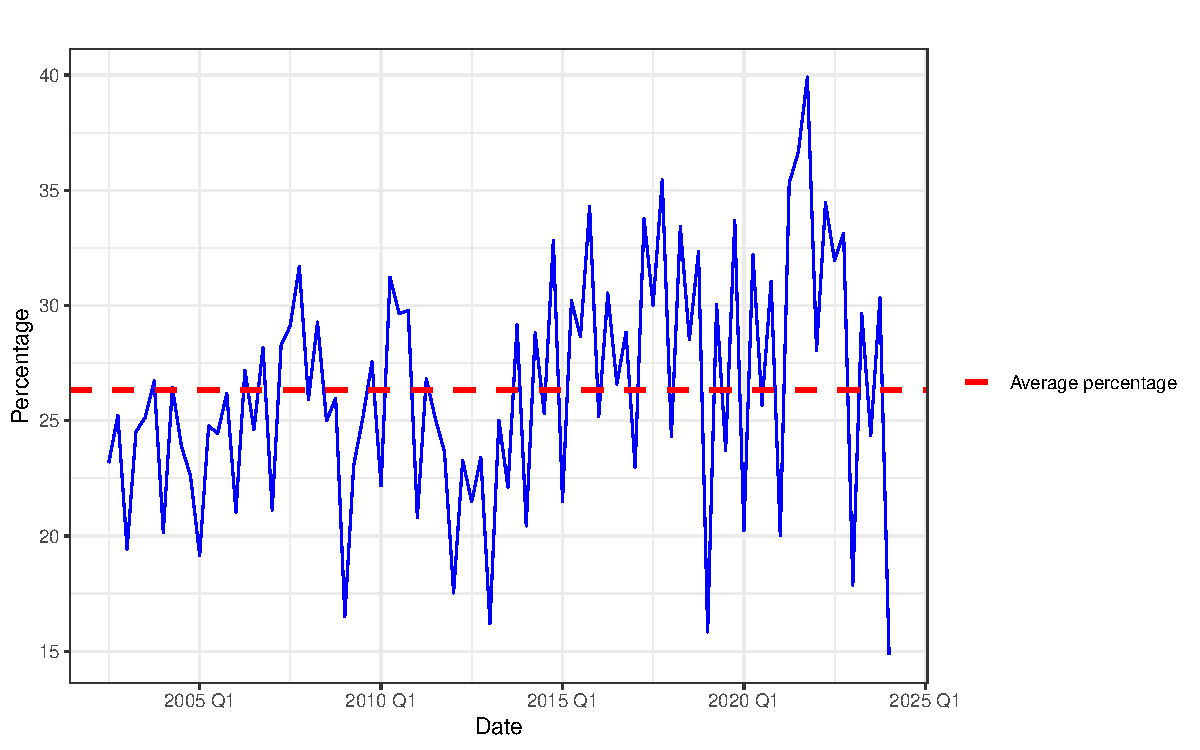
\includegraphics{Report_files/figure-pdf/fig-taxrevenue-1.pdf}

}

\caption{\label{fig-taxrevenue}Percentage of Victoria's Tax Revenue from
Land Transfer Duty}

\end{figure}%

Additionally, Victoria's tax revenue heavily relies on land transfer
duty. As shown in Figure~\ref{fig-taxrevenue}, over the past 20 years,
on average, land transfer duty accounts for \textbf{27\%} of Victoria's
tax revenue. Despite its perceived inequity and various exemptions
designed to aid homebuyers, abolishing this duty remains challenging due
to the need for equivalent revenue replacement. If this duty is removed,
the government will need to introduce one or more new taxes to generate
equivalent revenue.

To balance the need for sufficient tax income without discouraging
property transactions, \emph{the Department of Treasury and Finance}
(\textbf{DTF}) has been supporting the provision of better advice to the
government on policy adjustments, subsidies, exemptions, and
restrictions by delivering evidence-based insights. Accurate forecasts
of land transfer duty, both short-term (\emph{1 to 3 months}) and
long-term (\emph{12 months}), are essential for these decisions.

This report introduces a new forecasting methodology aimed at improving
the accuracy of these predictions. By employing forecast reconciliation
and combining cross-sectional and temporal hierarchies, we aim to
provide the \emph{Department of Treasury and Finance} with more reliable
forecasts to inform policy-making. The primary advantage of this
methodology is that it produces forecasts at various aggregation levels
within both cross-sectional and temporal hierarchies, allowing for the
inclusion of unique characteristics of different nodes. Our results use
monthly land transfer duty data, covering the period from July 2013 to
March 2024.

Our project employs three forecasting models, including vector error
correction model (VECM), vector autoregressive model (VAR) and
autoregressive integrated moving average (ARIMA). For the model fitting
process, we include three macroeconomic indicators and property market
indices, which are sales, home value index and lending provided by the
Australian Bureau of Statistics (ABS) and CoreLogic. The rationale for
selecting these three explanatory variables is that the best-performing
models used by the \emph{Department of Treasury and Finance} also employ
them.

To assess the forecast performance, we use time series cross-validation
to ensure that the corresponding training set consists only of
observations that occurred prior to the observation that forms the test
set. The length of the first training set contains 108 months of data
(equivalent to 9 years) and increase the size of successive training
sets by one month. As a result, there will be 10 testing sets with 1 to
12-step-ahead forecasts. We then computed accuracy measures,
specifically root mean squared errors (RMSE) and mean absolute
percentage errors (MAPE), for all forecasts, and finally averaged them
across the 10 sets.

Overall, the results suggest that VECM, particularly when using
cross-temporal reconciliation, consistently outperforms ARIMA. Temporal
hierarchies contribute more to accuracy improvements than
cross-sectional hierarchies. The reconciled forecasts from VECM exhibit
lower RMSE and MAPE compared to the \emph{Department of Treasury and
Finance}'s forecasts, underscoring the efficacy of the proposed
approach.

The rest of the paper is organized as follows. Section 3 includes
exploratory data analysis (EDA). Section 4 explores the forecasting
methods covered in detail. Section 5 discusses the detailed time series
cross-validation process adopted for this project. Section 6 presents
the main results and their implementation. Section 7 concludes the study
and offers recommendations.

\section{Exploratory Data Analysis
(EDA)}\label{exploratory-data-analysis-eda}

In this section, we conduct a detailed Exploratory Data Analysis (EDA)
for the total land transfer duty and all its disaggregated levels, as
well as for other included exploratory variables. Each of the three
exploratory variables serves as a measure of property market performance
and will have interrelations with land transfer duty.

\subsection{Time series analysis}\label{sec-tsanalysis}

For this project, the total land transfer duty is divided into
residential and non-residential categories. The non-residential land
transfer duty is further disaggregated into commercial, industrial, and
other categories. Figure~\ref{fig-crosssec1} provides an overview of the
cross-sectional hierarchical structure.

\begin{figure}

\centering{

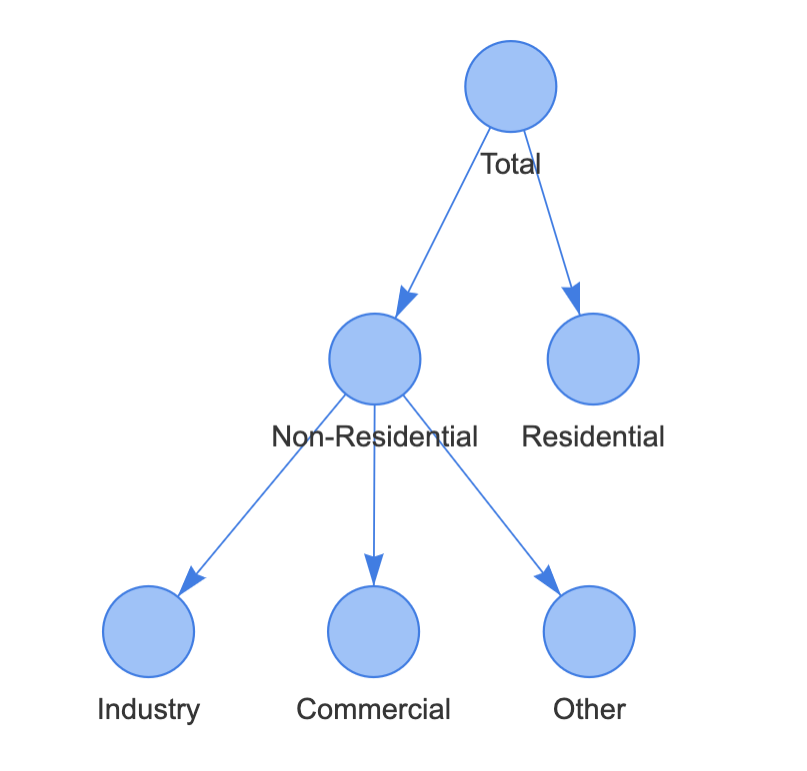
\includegraphics[width=0.65\textwidth,height=\textheight]{image/cross_sec.png}

}

\caption{\label{fig-crosssec1}Cross-sectional hierarchy}

\end{figure}%

\subsubsection{Total Land Transfer Duty}\label{total-land-transfer-duty}

\begin{figure}

\centering{

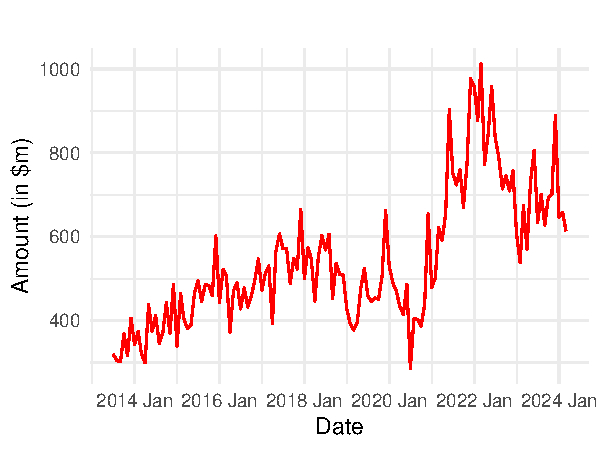
\includegraphics{Report_files/figure-pdf/fig-trend-1.pdf}

}

\caption{\label{fig-trend}Time plot of Land Transfer Duty in Victoria
over time}

\end{figure}%

Figure~\ref{fig-trend} demonstrates an upward, non-linear trend, showing
that the value of land transfer duty has generally increased over the
ten-year period. Note that, due to the outbreak of Covid-19, total land
transfer duty experienced a significant decline, reaching a low of 286.2
million in June 2020. Subsequently, it rebounded to an unprecedented
peak of 1.013 billion in March 2022. This trend can be attributed to
multiple rate cuts by the Reserve Bank of Australia, which initially
aimed to stabilize the real estate sector and subsequently stimulated
demand. Additionally, there is a noticeable increase in variability,
particularly in recent years, indicating more pronounced fluctuations in
the values. This increasing volatility suggests that a transformation of
the data may be necessary to better analyze and model these trends.

\begin{figure}

\centering{

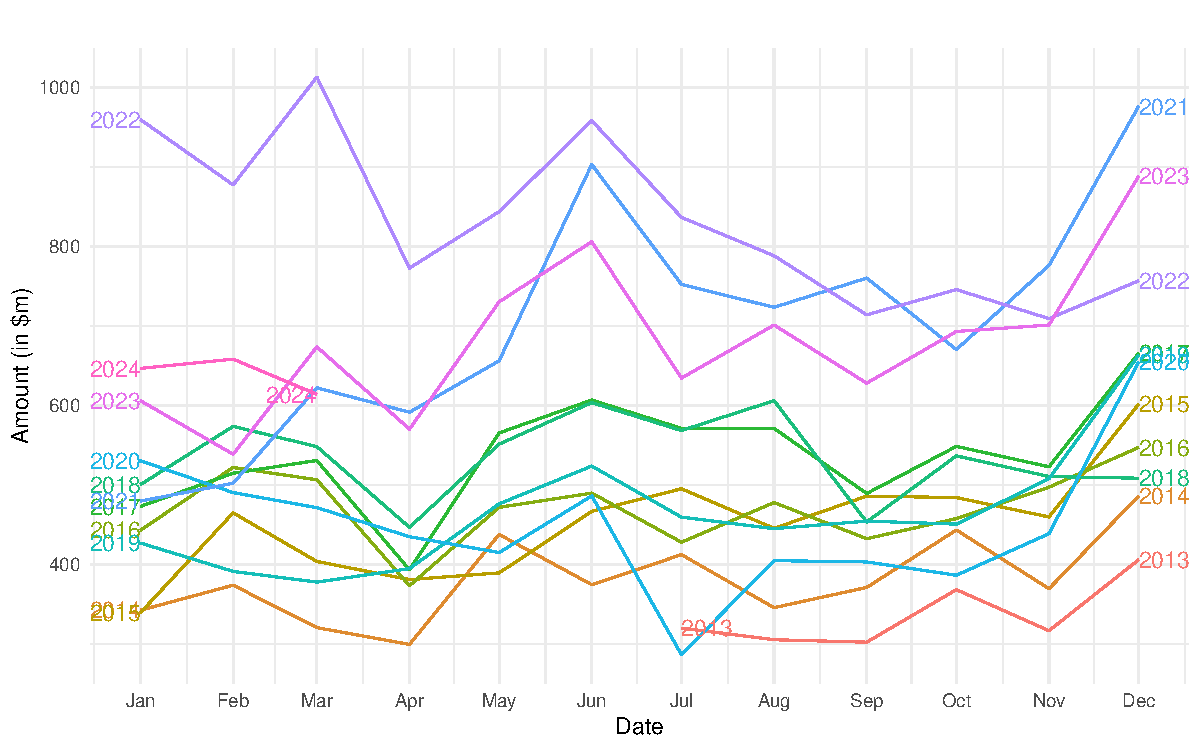
\includegraphics{Report_files/figure-pdf/fig-sspattern-1.pdf}

}

\caption{\label{fig-sspattern}Seasonal plot of Land Transfer Duty in
Victoria}

\end{figure}%

Considering the seasonal patterns of land transfer duty, referring to
Figure~\ref{fig-sspattern}, it is clear that there is a large jump in
land transfer duty in June and December each year. This may be
attributed to June being the end of financial year, when buyers rush to
complete transactions to take advantage of tax benefits, financial
reporting, while December being the end of calender year, when many
individuals aim to complete transactions before the holiday season.
Figure~\ref{fig-sspattern} also shows that there is a decrease in April
each year.

\begin{figure}

\centering{

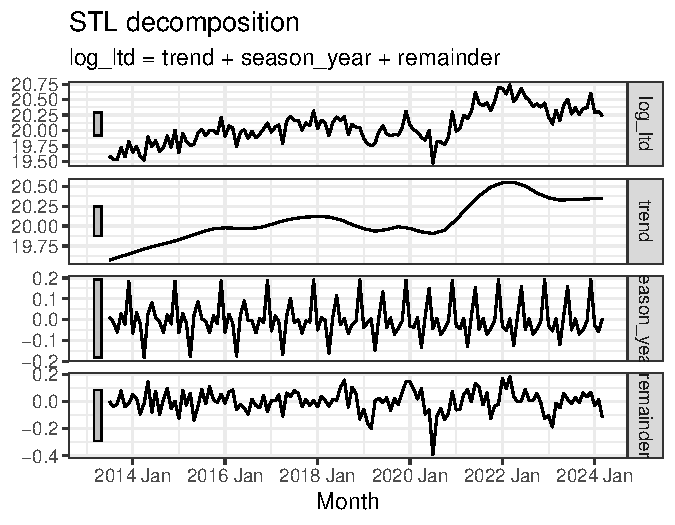
\includegraphics{Report_files/figure-pdf/fig-dcmp-1.pdf}

}

\caption{\label{fig-dcmp}Log of total Land Transfer Duty in Victoria
(top) and its three additive components.}

\end{figure}%

\begin{figure}

\centering{

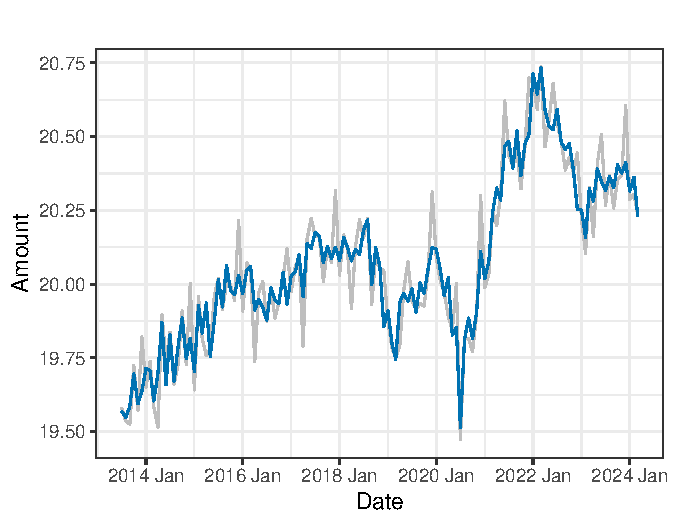
\includegraphics{Report_files/figure-pdf/fig-ssadj-1.pdf}

}

\caption{\label{fig-ssadj}Seasonally adjusted of log Land Transfer Duty
(blue) and the original data (grey)}

\end{figure}%

Figure~\ref{fig-dcmp} shows that there is a seasonal pattern for log
transformed land transfer duty, which agrees with what indicated from
Figure~\ref{fig-sspattern}. The grey bars positioned to the left of each
panel illustrate the relative scales of the components. Although each
grey bar represents an same length, their sizes differ due to the
distinct scales of the plots. The prominent grey bar in the seasonal
panel indicates that the variation in the seasonal component is the
smallest when compared to the overall variation in the data.

Moreover, Figure~\ref{fig-dcmp} demonstrates that after applying a log
transformation, the variability becomes more consistent. However, the
relatively small grey bar to the left of the remainder panel indicates
that some heterogeneity persists.

The grey line in Figure~\ref{fig-ssadj} represents the log-transformed
total land transfer duty, while the blue line represents the seasonally
adjusted log-transformed total land transfer duty.
Figure~\ref{fig-ssadj} suggests that by adjusting for the seasonal
pattern, some local peaks and troughs have been smoothed out.

\subsubsection{Residential property land transfer
duty}\label{residential-property-land-transfer-duty}

\begin{figure}

\centering{

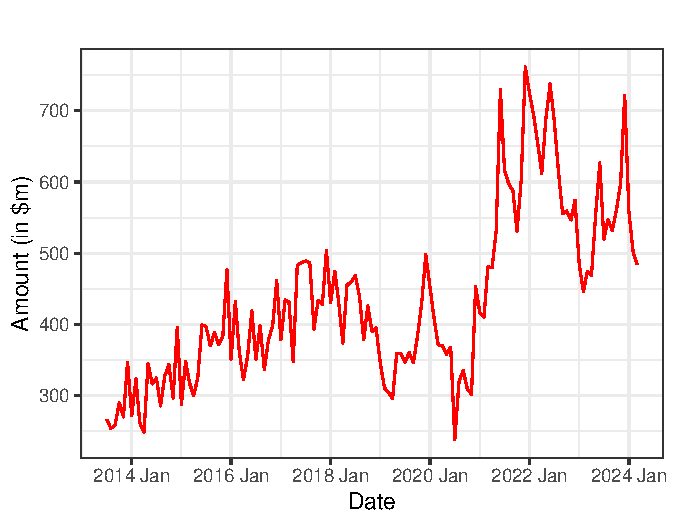
\includegraphics{Report_files/figure-pdf/fig-restrend-1.pdf}

}

\caption{\label{fig-restrend}Time plot of Residential property Land
Transfer Duty in Victoria}

\end{figure}%

Figure~\ref{fig-restrend} illustrates a non-linear upward trend in
residential property land transfer duty, closely mirroring the overall
trend in total land transfer duty. The figure also reflects the impact
of the Covid-19 pandemic, with a significant decline to a low of 238.1
million in June 2020, followed by a rebound to an all-time high of 761.4
million in December 2021. This pattern is attributable to the fact that
residential property comprises the largest portion of land transfer
duty. These findings suggest that residential property remains a crucial
component of the market, likely reflecting trends in housing demand and
price fluctuations. Additionally, there is an increase in variability
over time, which also suggests a transformation of the data.

\begin{figure}

\centering{

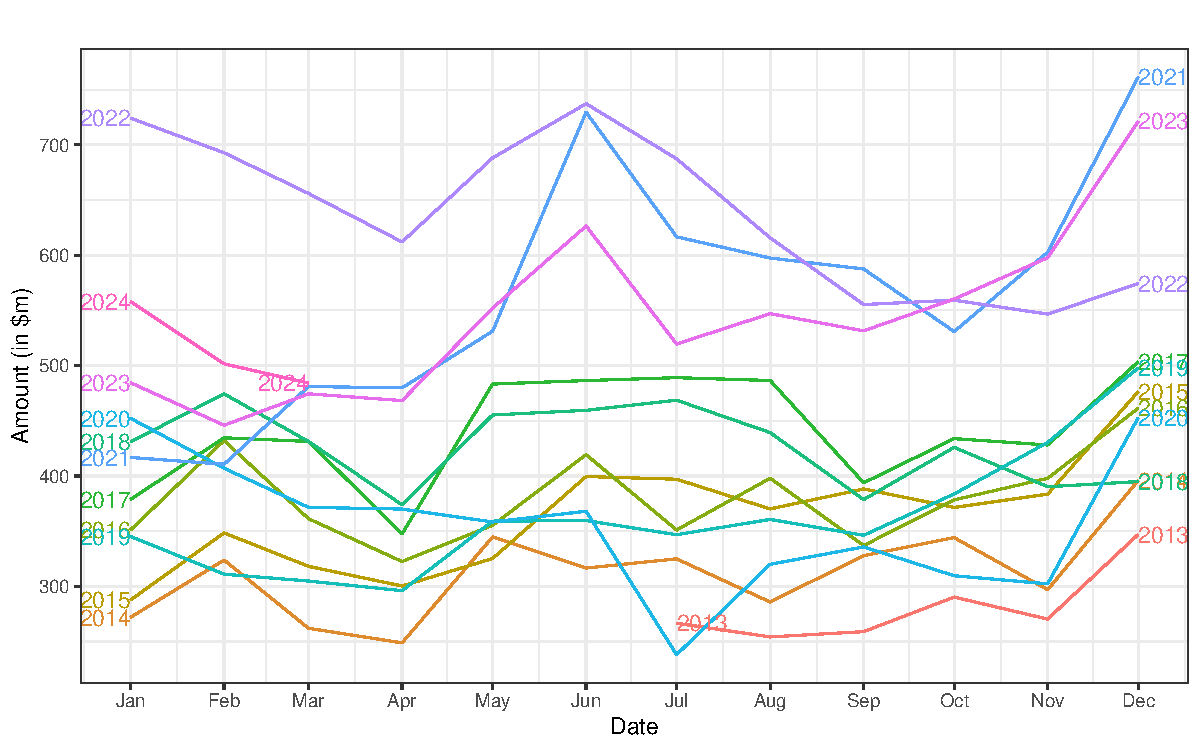
\includegraphics{Report_files/figure-pdf/fig-resspattern-1.pdf}

}

\caption{\label{fig-resspattern}Seasonal plot of Residential property
Land Transfer Duty in Victoria}

\end{figure}%

Since as discussed above, we expect residential land transfer duty also
mirrors the seasonal pattern of total land transfer duty, which is shown
in Figure~\ref{fig-resspattern}. There is also a large jump in land
transfer duty in June and December each year, which can be explained by
the same reason.

\subsubsection{Non-residential property land transfer
duty}\label{non-residential-property-land-transfer-duty}

\begin{figure}

\centering{

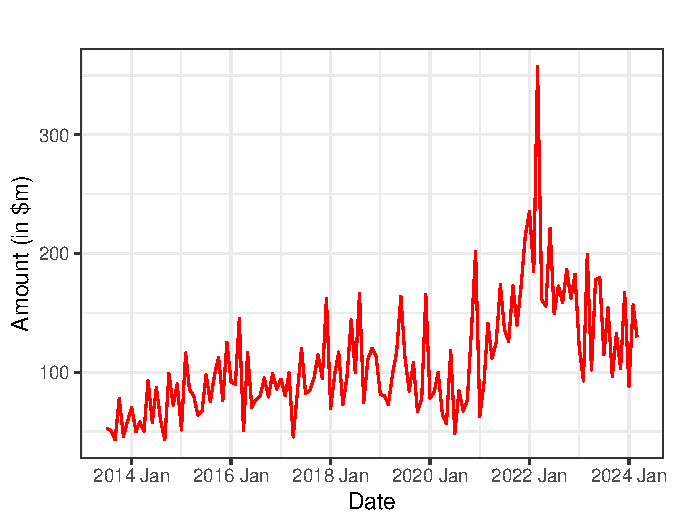
\includegraphics{Report_files/figure-pdf/fig-nonrestrend-1.pdf}

}

\caption{\label{fig-nonrestrend}Time plot of Non-residential property
Land Transfer Duty in Victoria}

\end{figure}%

Figure~\ref{fig-nonrestrend} shows a markedly different pattern in
non-residential property land transfer duty compared to total and
residential property duty. While non-residential duty reached an
all-time high of 357.2 million in March 2022 post-Covid-19, it lacks a
consistent long-term growth trend, exhibiting significant variability.
Moreover, the sudden drop after reaching its all time high in March 2022
may suggest that non-residential sector reacts more significantly to
changes in the cash rate than the residential sector.

\begin{figure}

\centering{

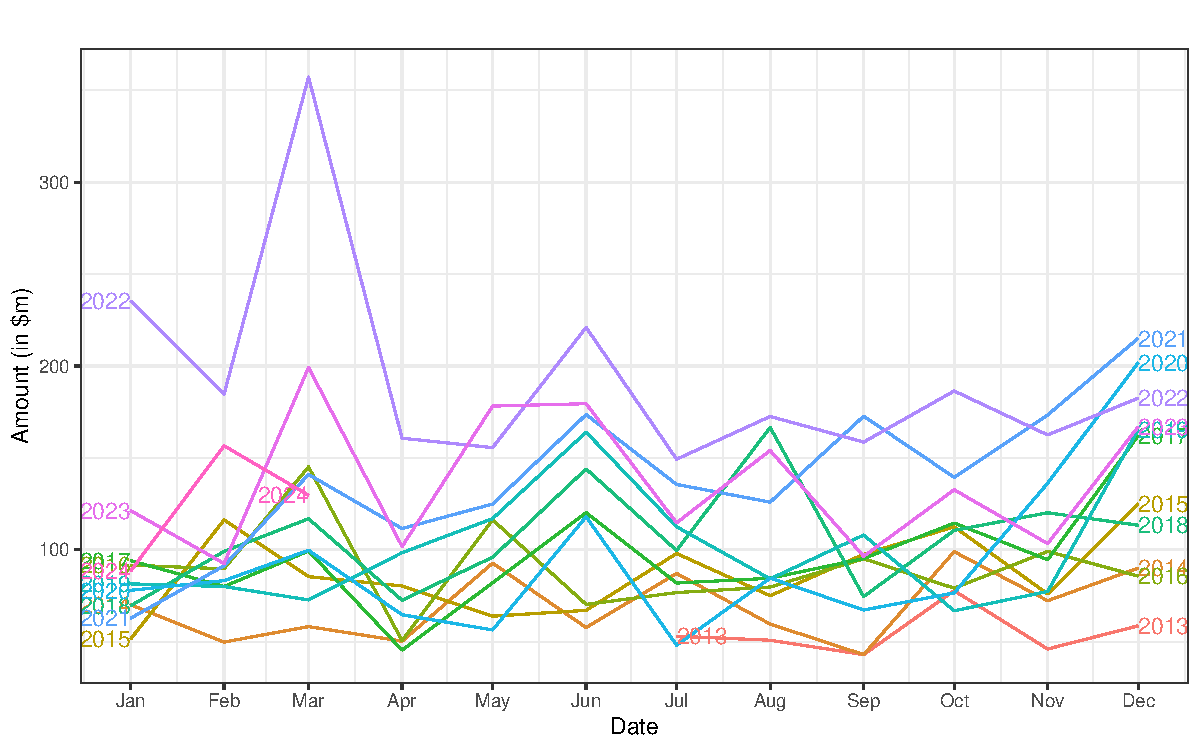
\includegraphics{Report_files/figure-pdf/fig-nonresspattern-1.pdf}

}

\caption{\label{fig-nonresspattern}Seasonal plot of Non-residential
property Land Transfer Duty in Victoria}

\end{figure}%

Figure~\ref{fig-nonresspattern} also shows an increase in June and
December each year. Although the magnitude of change is smaller compared
to total and residential property land transfer duty, the increasing
pattern is more consistent across all years.

\subsubsection{Commercial property land transfer
duty}\label{commercial-property-land-transfer-duty}

\begin{figure}

\centering{

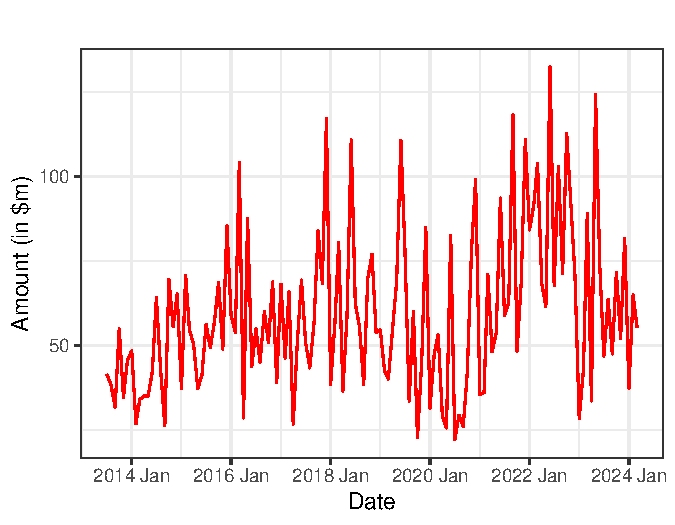
\includegraphics{Report_files/figure-pdf/fig-commtrend-1.pdf}

}

\caption{\label{fig-commtrend}Time plot of Commercial property Land
Transfer Duty in Victoria}

\end{figure}%

Figure~\ref{fig-commtrend} demonstrates the fluctuations in commercial
property land transfer duty from 2014 to 2024. The plot also exhibits
significant variability, with several peaks and troughs over the
observed period, ranging from 22.1 million to 132.4 million. Notably,
the commercial land transfer duty reached its highest levels in early
2022, reflecting a post-Covid-19 recovery. However, unlike the
residential sector, the commercial property sector does not show a
consistent long-term growth trend.

\begin{figure}

\centering{

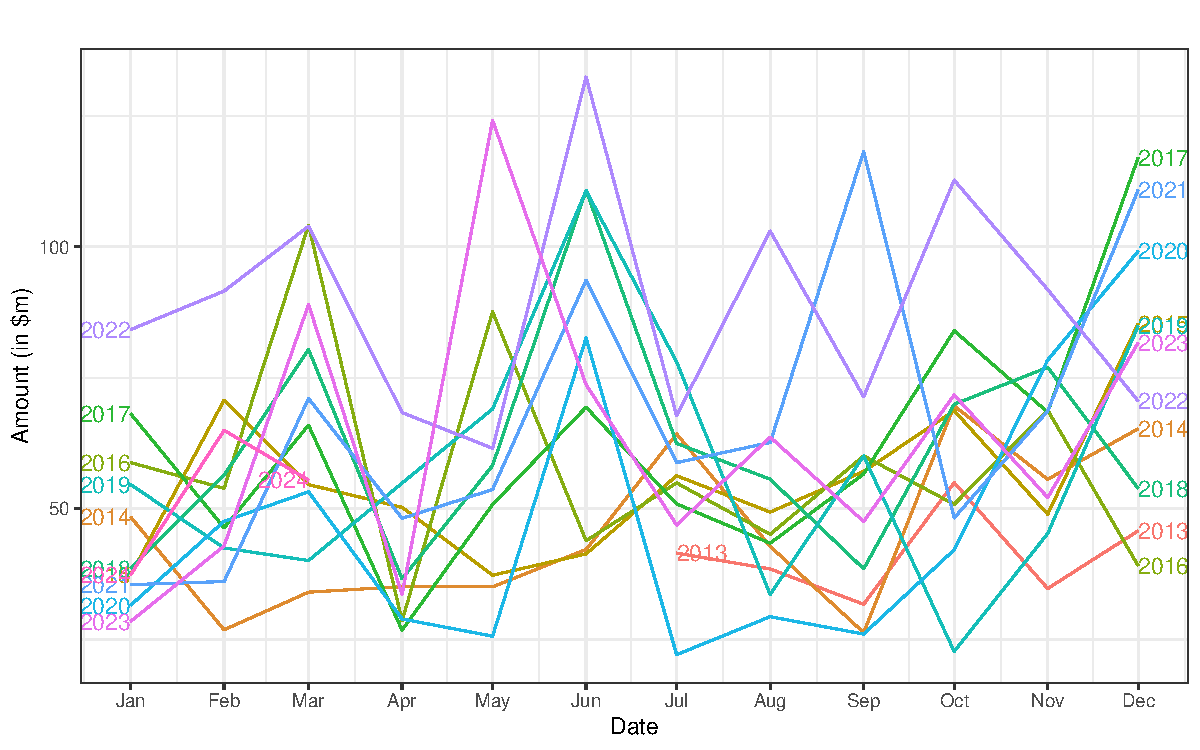
\includegraphics{Report_files/figure-pdf/fig-commspattern-1.pdf}

}

\caption{\label{fig-commspattern}Seasonal plot of Commerical property
Land Transfer Duty in Victoria}

\end{figure}%

Figure~\ref{fig-commspattern} demonstrates various increases throughout
the year, in March, May, June and December, highlighting significant
fluctuations throughout the year. Moreover, while some years display
consistent seasonal patterns, others show irregular fluctuations.

\subsubsection{Industrial property land transfer
duty}\label{industrial-property-land-transfer-duty}

\begin{figure}

\centering{

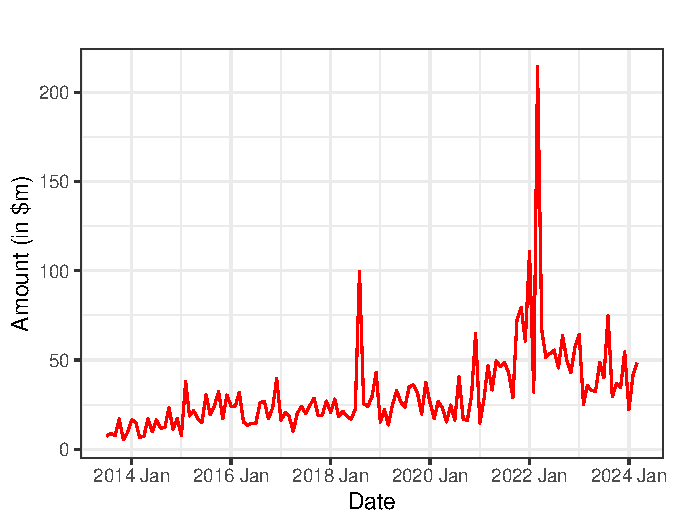
\includegraphics{Report_files/figure-pdf/fig-indtrend-1.pdf}

}

\caption{\label{fig-indtrend}Time plot of Industrial property Land
Transfer Duty in Victoria}

\end{figure}%

Figure~\ref{fig-indtrend} shows a more stable variability compared to
residential or total land transfer duty, with less pronounced
fluctuations, apart from notable peaks observed in mid-2018 and March
2022. Overall, the trend is non-increasing, indicating a lack of
long-term growth. The industrial sector has collected land transfer duty
between 5.2 million and 214.4 million, highlighting some large-scale
industrial transactions or developments during certain periods. These
characteristics suggest that while industrial property transactions
exhibit periodic spikes, they generally maintain a steady pattern
without significant upward or downward trends.

\begin{figure}

\centering{

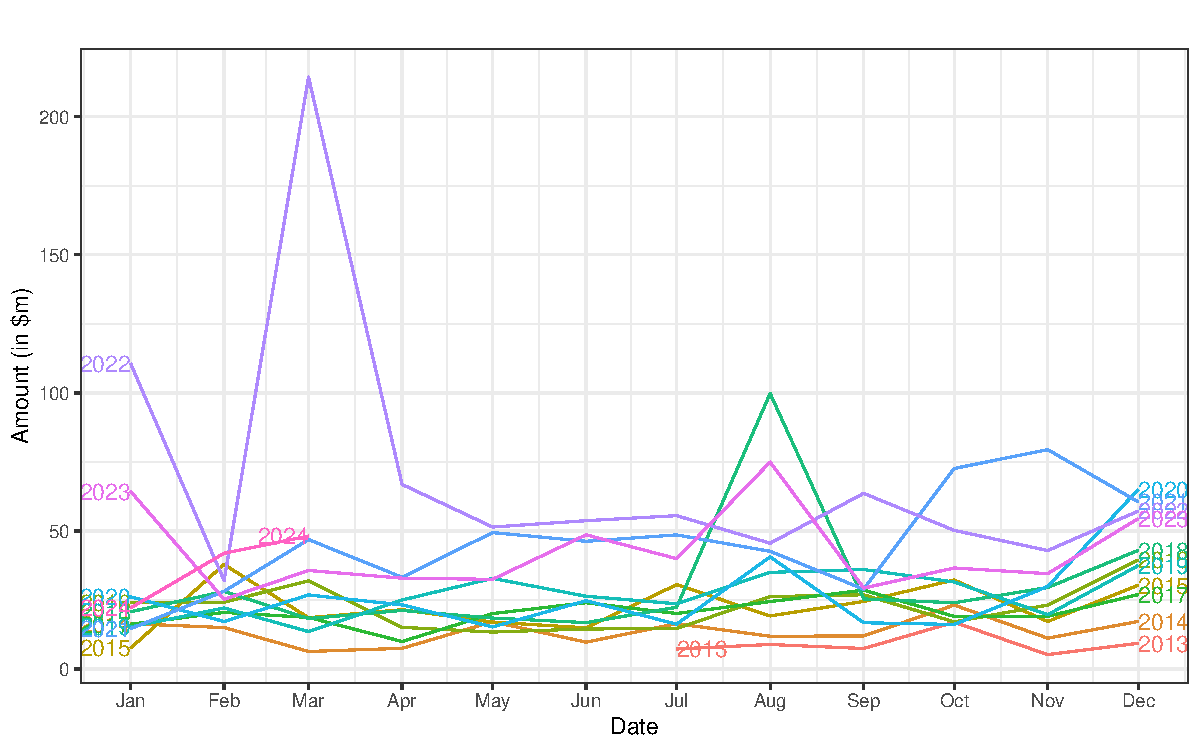
\includegraphics{Report_files/figure-pdf/fig-indspattern-1.pdf}

}

\caption{\label{fig-indspattern}Seasonal plot of Industrial property
Land Transfer Duty in Victoria}

\end{figure}%

Apart from slight increases in August and December each year,
Figure~\ref{fig-indspattern} shows that there is no clear indication of
seasonal pattern.

\subsubsection{Other property land transfer
duty}\label{other-property-land-transfer-duty}

\begin{figure}

\centering{

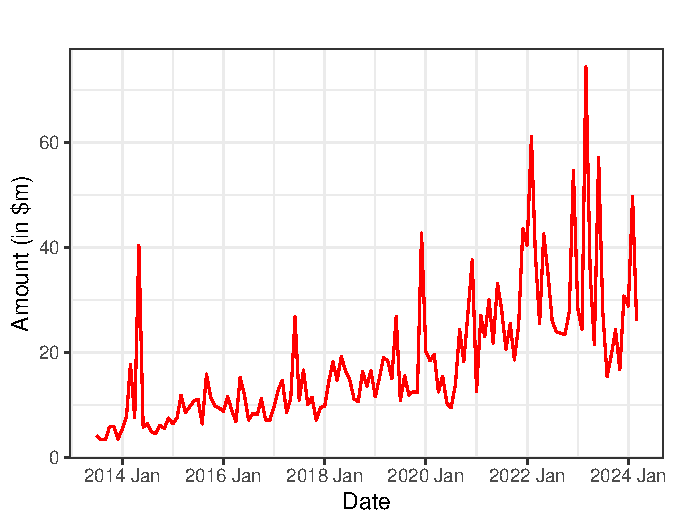
\includegraphics{Report_files/figure-pdf/fig-othertrend-1.pdf}

}

\caption{\label{fig-othertrend}Time plot of Other type property Land
Transfer Duty in Victoria}

\end{figure}%

Figure~\ref{fig-othertrend} shows a non-linear increasing trend in other
type property land transfer duty, including agricultural with different
variability over time and irregular peaks. Contributions from these
sectors range from 3.3 million to 74.5 million, indicating sporadic
activity that may correspond with specific market or economic
conditions.

\begin{figure}

\centering{

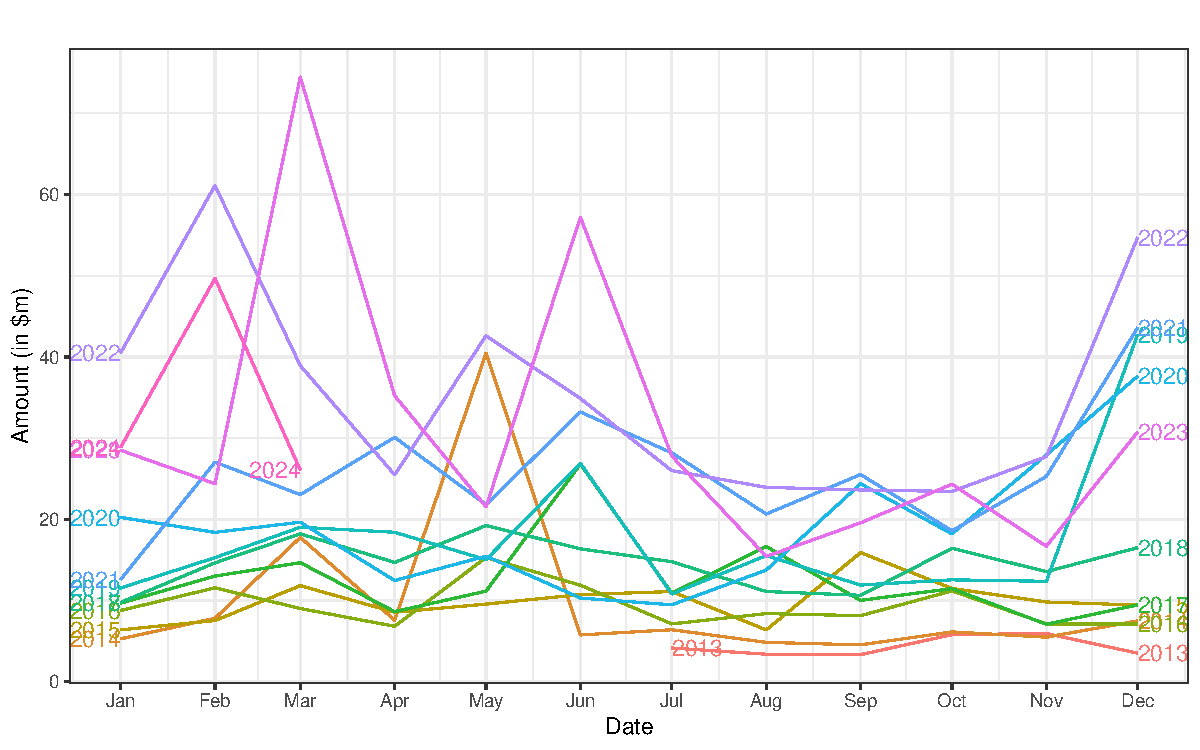
\includegraphics{Report_files/figure-pdf/fig-otherspattern-1.pdf}

}

\caption{\label{fig-otherspattern}Seasonal plot of Other type property
Land Transfer Duty in Victoria}

\end{figure}%

As shown in Figure~\ref{fig-otherspattern}, the seasonal pattern is
quite irregular across all years, but there is a consistent increase
observed in December for the past several years from 2020.

\subsubsection{Sales}\label{sales}

The sales variable indicates the number of properties sold in Victoria,
measured in units at the contract date for all types of residential
dwellings.

\begin{figure}

\centering{

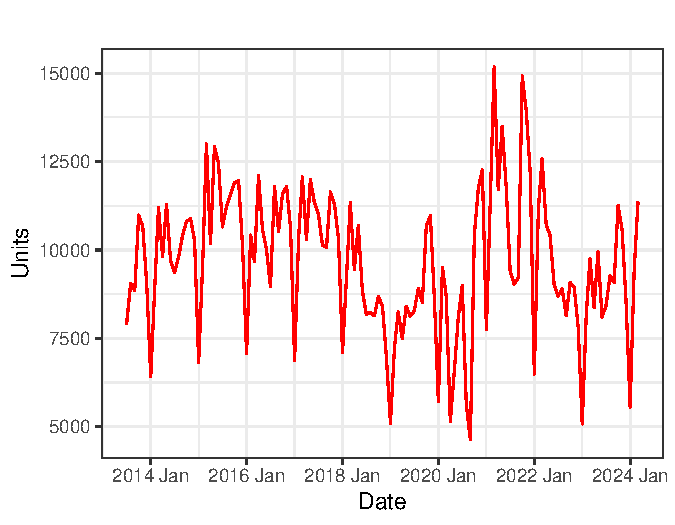
\includegraphics{Report_files/figure-pdf/fig-salestrend-1.pdf}

}

\caption{\label{fig-salestrend}Time Plot of Units of Properties Sold in
Victoria}

\end{figure}%

Figure~\ref{fig-salestrend} shows a non-linear trend, and strong
fluctuations in sales units over the ten-year period from January 2014
to January 2024. The plot exhibits considerable variability with both
high and low peaks scattered throughout the timeline. The values range
from approximately 5000 to over 15000, indicating significant changes in
sales units.

In recent years, there is a noticeable increase in variability,
particularly around 2020 and onwards. This increasing volatility
indicates that a transformation of the data may be necessary to better
analyze and model these trends.

\begin{figure}

\centering{

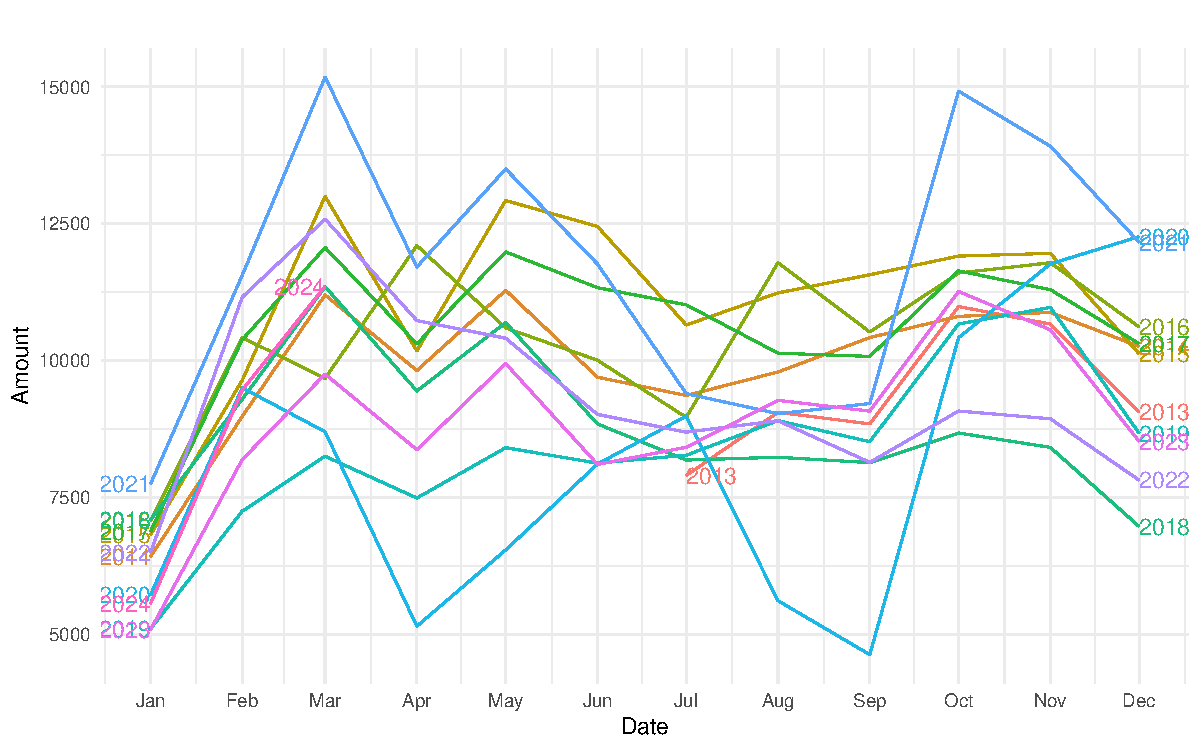
\includegraphics{Report_files/figure-pdf/fig-salessspattern-1.pdf}

}

\caption{\label{fig-salessspattern}Seasonal plot of Units of Properties
Sold in Victoria}

\end{figure}%

Figure~\ref{fig-salessspattern} exhibits a significant decline in sales
units in December, followed by a trough in January each year. This trend
contrasts with the observed increase in total land transfer duty in
December, as depicted in the seasonal plot in
Figure~\ref{fig-sspattern}. This discrepancy can be attributed to the
fact that, despite the reduction in the number of sales units, the
properties sold during this period are typically of higher value,
thereby driving up the total land transfer duty.

\begin{figure}

\centering{

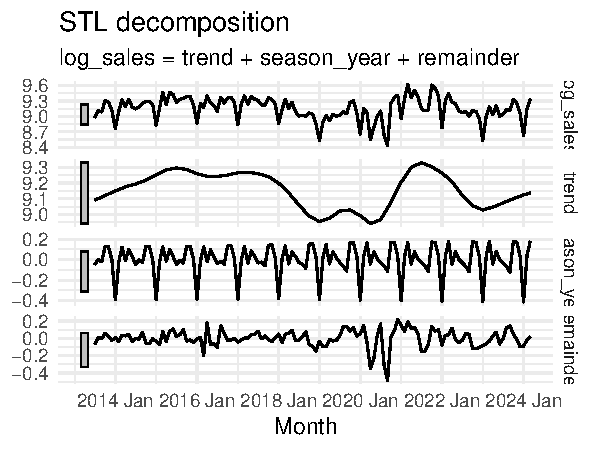
\includegraphics{Report_files/figure-pdf/fig-salesdcmp-1.pdf}

}

\caption{\label{fig-salesdcmp}Log of Units of Properties Sold in
Victoria (Top) and Its Three Additive Components}

\end{figure}%

\begin{figure}

\centering{

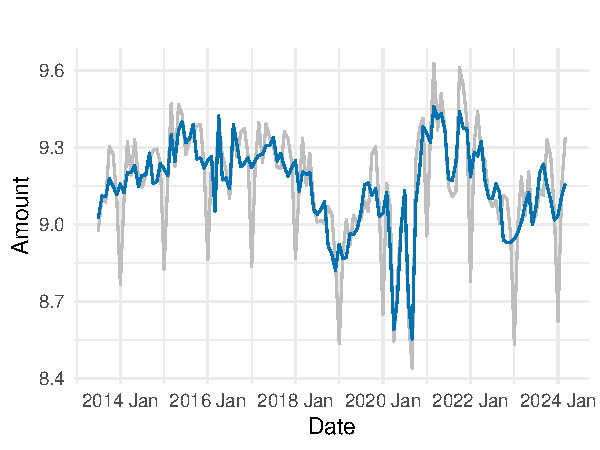
\includegraphics{Report_files/figure-pdf/fig-salesssadj-1.pdf}

}

\caption{\label{fig-salesssadj}Seasonally adjusted of log of Units of
Properties Sold in Victoria (blue) and the original data (grey).}

\end{figure}%

Figure~\ref{fig-salesdcmp} indicates a seasonal pattern for
log-transformed sales, which agrees with
Figure~\ref{fig-salessspattern}. However, the large grey bar in the
seasonal panel indicates that the variation in the seasonal component is
the smallest when compared to the overall variation in the data.

Moreover, Figure~\ref{fig-salesdcmp} demonstrates that after applying a
log transformation, the variability becomes more consistent, although
some heterogeneity still remains.

The grey line in Figure~\ref{fig-salesssadj} represents the original
log-transformed sales, while the blue line represents the seasonally
adjusted log-transformed sales. Figure~\ref{fig-salesssadj} suggests
that there is a huge difference between seasonally adjusted sales and
original sales, especially in periodic drops.

\subsubsection{Home Value Index}\label{home-value-index}

The Home Value Index aims to measure monthly movements in the value of
Australian housing markets.

\begin{figure}

\centering{

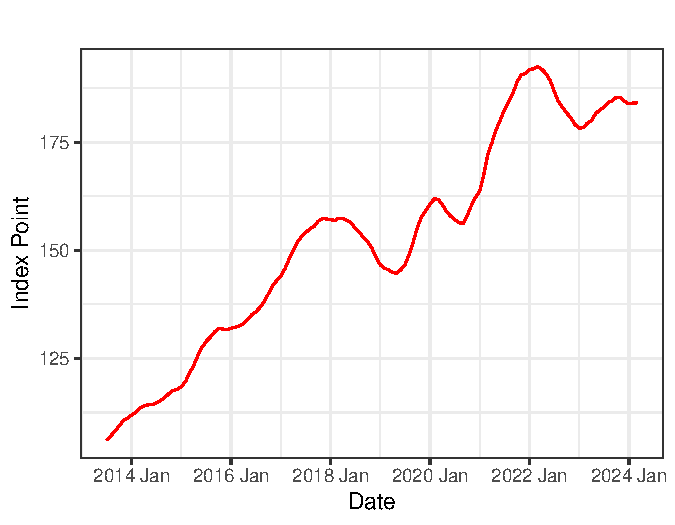
\includegraphics{Report_files/figure-pdf/fig-hvitrend-1.pdf}

}

\caption{\label{fig-hvitrend}Time plot of Home Value Index in Victoria
over time}

\end{figure}%

Figure~\ref{fig-hvitrend} illustrates an increasing trend, with some
considerable variability throughout the timeline. There is no clear sign
of seasonal pattern in home value index.

\subsubsection{Lending}\label{lending}

Lending is the new borrower-accepted finance commitments for housing,
personal and business loans from Australian Bureau Statistics (ABS),
relating to all types of residential transactions.

\begin{figure}

\centering{

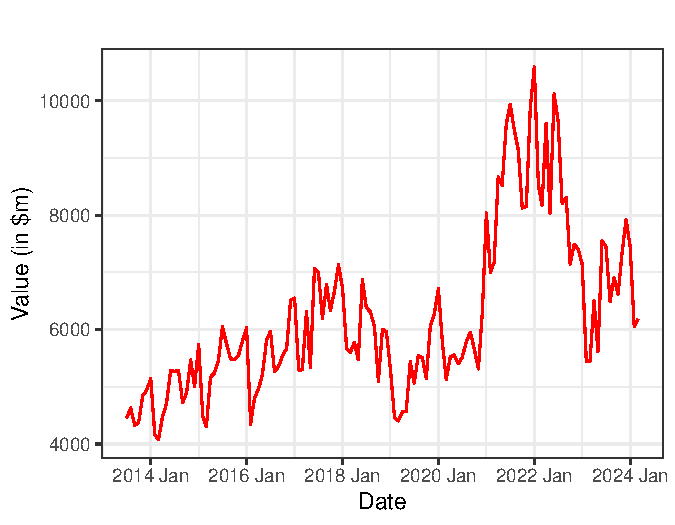
\includegraphics{Report_files/figure-pdf/fig-lendingtrend-1.pdf}

}

\caption{\label{fig-lendingtrend}Time plot of Lending in Victoria over
time}

\end{figure}%

Figure~\ref{fig-lendingtrend} shows an overall increasing trend over
time with clear seasonal pattern for lending.

\subsection{Dealing with seasonality}\label{dealing-with-seasonality}

As discussed in Section~\ref{sec-tsanalysis}, it is evident that many
time series exhibit seasonal patterns. Given the limitations of Vector
Error Correction Models (VECM) in adequately modeling these seasonal
fluctuations, we propose a methodological adjustment. Specifically, we
will decompose the time series into seasonally adjusted components and
explicit seasonal factors. This decomposition allows us to apply VECM to
the seasonally adjusted data. Subsequently, we will conduct independent
forecasts for both the seasonally adjusted data and the seasonal
components. The final step involves the reconciliation of these
forecasts then integrating them.

\subsection{Cointegration Analysis for modelling}\label{sec-coint}

Based on the observations from Figure~\ref{fig-trend}, which illustrates
the trend and increasing variance pattern in land transfer duty while
other disaggregated levels of land transfer duty exhibit either a trend
or seasonal pattern, we can conclude that these series are
non-stationary. The same findings apply to the three exploratory
variables.

Furthermore, to justify the use of the Vector Error Correction Model
(VECM) by the \emph{Department of Treasury and Finance}, it is essential
to test for the presence of cointegration patterns (or long-term
equilibrium relationships) among these three series.

The Johansen procedure with the trace test statistic will be employed to
test for cointegration between log transformed of land transfer duty,
sales, and the home value index series. This procedure tests the null
hypothesis that no cointegration relationship exists among the series.

\begin{table}

\caption{\label{tbl-jotest}Johansen test result}

\centering{

\centering
\begin{tabular}{l|l|r|r|r|r}
\hline
  & Rank & Test Statistic & 10\% & 5\% & 1\%\\
\hline
r <= 2 | & r <= 2 & 2.30 & 6.50 & 8.18 & 11.65\\
\hline
r <= 1 | & r <= 1 & 17.34 & 15.66 & 17.95 & 23.52\\
\hline
r = 0  | & r = 0 & 57.15 & 28.71 & 31.52 & 37.22\\
\hline
\end{tabular}

}

\end{table}%

The test results, as shown in Table~\ref{tbl-jotest}, using 3 lags as
chosen by the DTF, allow us to reject the null hypothesis that
\(r \leq 1\), yet we fail to reject the null hypothesis that
\(r \leq 2\) at 5\% level of significance. This suggests that among the
three variables, the rank of the matrix exceeds 2, indicating the
presence of at least two cointegration relationships.

Furthermore, a rank of 2 implies that we need a combination of at least
two time series to form a stationary series.

To create such a linear combination, we can utilize the components of
the eigenvector associated with the largest eigenvalue. According to the
Johansen test summary, the largest eigenvalue is approximately 0.27.
This corresponds to the eigenvectors components of \texttt{ltd\_total},
which is approximately equal to (1, -1.16, -1.39). By forming a linear
combination of the series using these eigenvector components, we can
achieve a stationary series.

\begin{figure}

\centering{

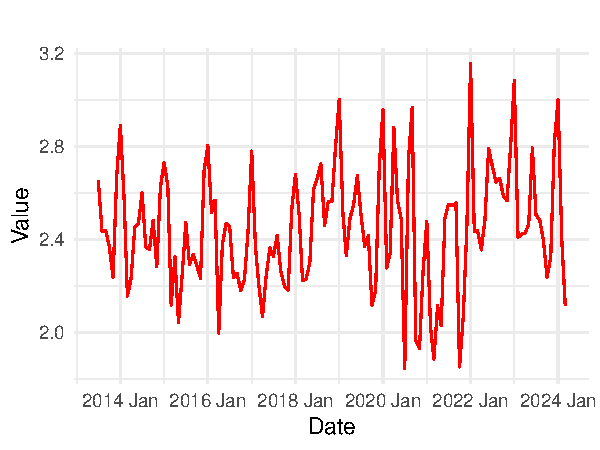
\includegraphics{Report_files/figure-pdf/fig-splot-1.pdf}

}

\caption{\label{fig-splot}Stationary series formed via a linear
combination of 3 time series}

\end{figure}%

As shown in Figure~\ref{fig-splot}, the linear combination appears to be
more stationary, although there remains a slight indication of varying
variances over time.

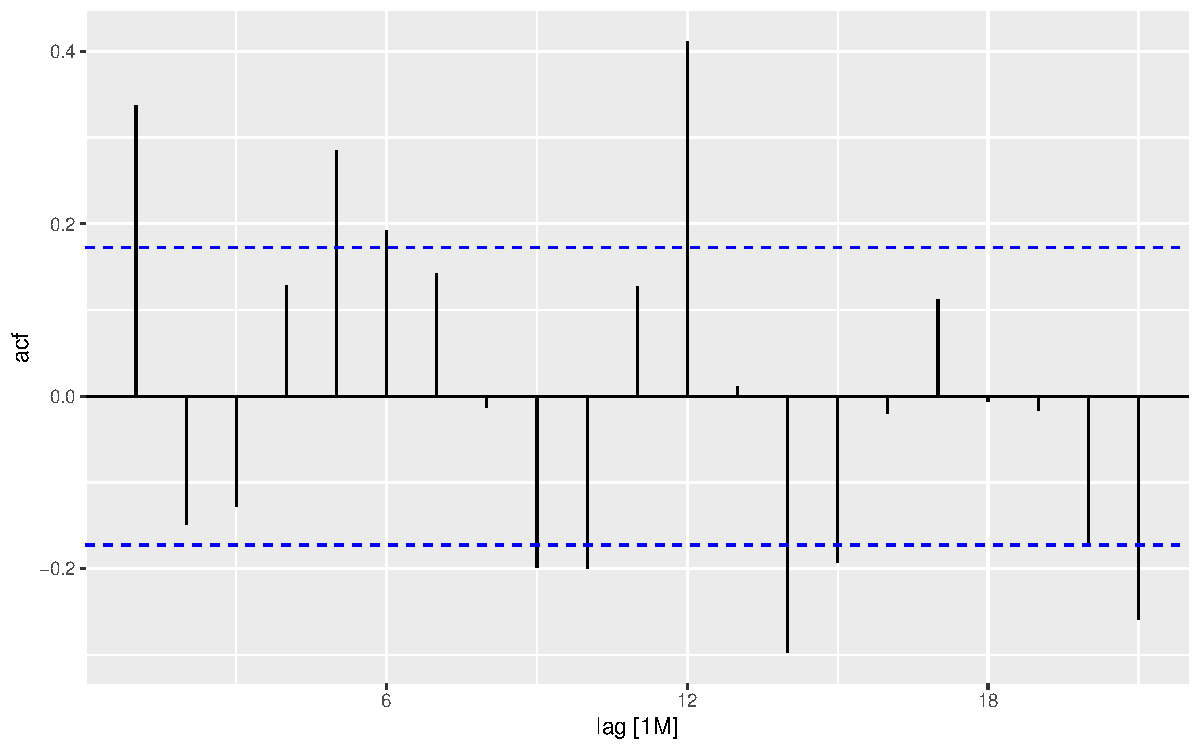
\includegraphics{Report_files/figure-pdf/unnamed-chunk-30-1.pdf}

Additionally, the p-value of 0.09 from the Augmented Dickey-Fuller (ADF)
test indicates that we can reject the null hypothesis of a unit root,
providing evidence of a stationary series formed from the linear
combination at the 10\% level of significance. Therefore, we can
conclude that it is appropriate to fit a Vector Error Correction Model
(VECM) to these three time series.

Since we will fit VECM to all the variables in the hierarchy, including
residential, non-residential, commercial, property and other, we will
perform the same procedure of cointegration analysis as above.

\begin{table}

\caption{\label{tbl-adftest}Johansen and ADF test for other type ltd}

\centering{

\centering
\begin{tabular}{l|r|r}
\hline
Variable & Johansen p-value & ADF p-value\\
\hline
ltd\_res & 2 & 0.06\\
\hline
ltd\_nonres & 2 & 0.23\\
\hline
ltd\_comm & 2 & 0.14\\
\hline
ltd\_ind & 2 & 0.17\\
\hline
ltd\_other & 2 & 0.13\\
\hline
\end{tabular}

}

\end{table}%

As shown in Table~\ref{tbl-adftest}, the null hypothesis that the linear
combination is non-stationary cannot be rejected for the variables
\texttt{ltd\_nonres}, \texttt{ltd\_comm}, \texttt{ltd\_ind}, and
\texttt{ltd\_other}. This finding suggests that alternative variables
may be required to appropriately fit the Vector Error Correction Model
(VECM) for these specific property categories in land transfer duty.

\section{Methodology}\label{methodology}

\subsection{Cross-sectional, temporal and cross-temporal
hierarchies}\label{cross-sectional-temporal-and-cross-temporal-hierarchies}

Upon analyzing the data characteristics and the disaggregation of LTD,
it becomes evident that a three-level hierarchical structure can be
established. There is utility in generating forecasts at various levels
of aggregation, driven by diverse reasons and objectives. For example,
each level of aggregation may exhibit distinct characteristics; for
instance, transactions involving residential properties might vary from
those involving non-residential properties due to differences in market
dynamics or market size for each property type.

In this context, total land transfer duty is divided into two
categories: residential and non-residential properties. Non-residential
properties are further disaggregated into three sub-categories:
commercial, industrial, and other, which predominantly includes
agricultural properties. In addition to the total land transfer duty for
all property types, the government and the \emph{Department of Treasury
and Finance} may also be interested in forecasts for each category and
sub-category. Figure~\ref{fig-crosssec} illustrates the cross-sectional
hierarchical structure of land transfer duty as discussed.

\begin{figure}

\centering{

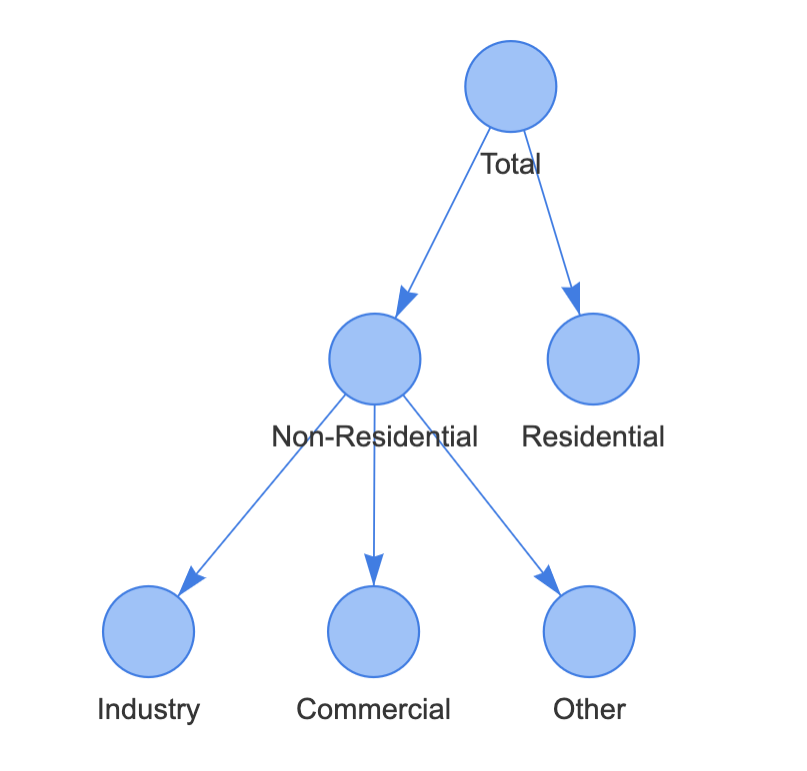
\includegraphics[width=0.65\textwidth,height=\textheight]{image/cross_sec.png}

}

\caption{\label{fig-crosssec}Cross-sectional hierarchy}

\end{figure}%

Given that this is a straightforward cross-sectional hierarchical
structure, we will also consider temporal hierarchies to further enhance
forecast accuracy. Land transfer duty is collected monthly, and
forecasts can be generated at bi-monthly, quarterly, four-monthly,
semi-annual, and annual frequencies. Various temporal hierarchies can be
constructed with monthly land transfer duty treated as the bottom level.
Figure~\ref{fig-temp} presents an example of temporal hierarchies with
monthly land transfer duty as the bottom level.

\begin{figure}

\centering{

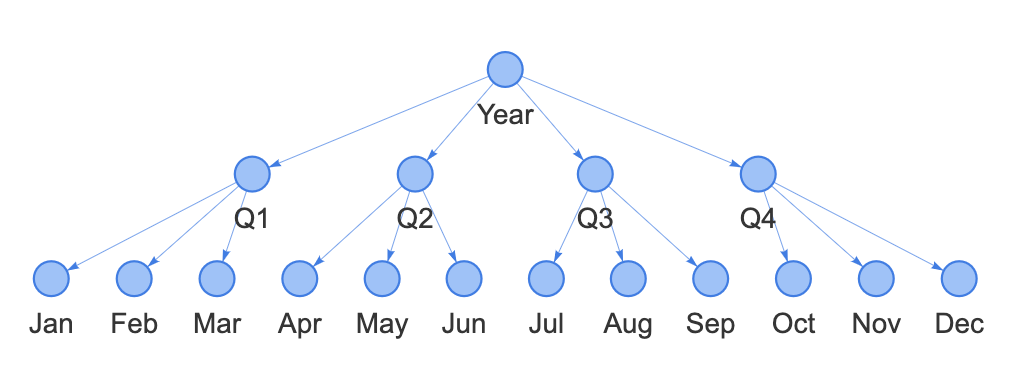
\includegraphics{image/temp.png}

}

\caption{\label{fig-temp}Temporal hierarchy}

\end{figure}%

Although forecasts using cross-sectional and temporal hierarchies have
demonstrated substantial improvements (\textcite{kourentzes2019cross}),
these approaches have typically been used separately. By combining
cross-sectional hierarchies and temporal hierarchies, referred to as
cross-temporal hierarchies, forecast accuracy can be further improved.
Moveover, another advantage of cross-temporal reconciled forecasts is
that it provides aligned short-term and long-term decision. If
cross-sectionally or temporally coherent forecasts are used
disjointedly, some outputs may not be directly useful, such as very
long-term forecasts at very disaggregate level, which is 2 years of
forecasts at other type of property land transfer duty level. Therefore,
one would have to post-process the forecasts further, for example
combining together multiple long-term disaggregate bottom level
forecasts (commerical, industrial, other) to produce long-term total
land transfer duty forecasts, which would then break the desired
coherence across all levels and time periods. Figure~\ref{fig-crosstemp}
from \textcite{kourentzes2019cross} shows an example of a cross-temporal
hierarchical structure.

\begin{figure}

\centering{

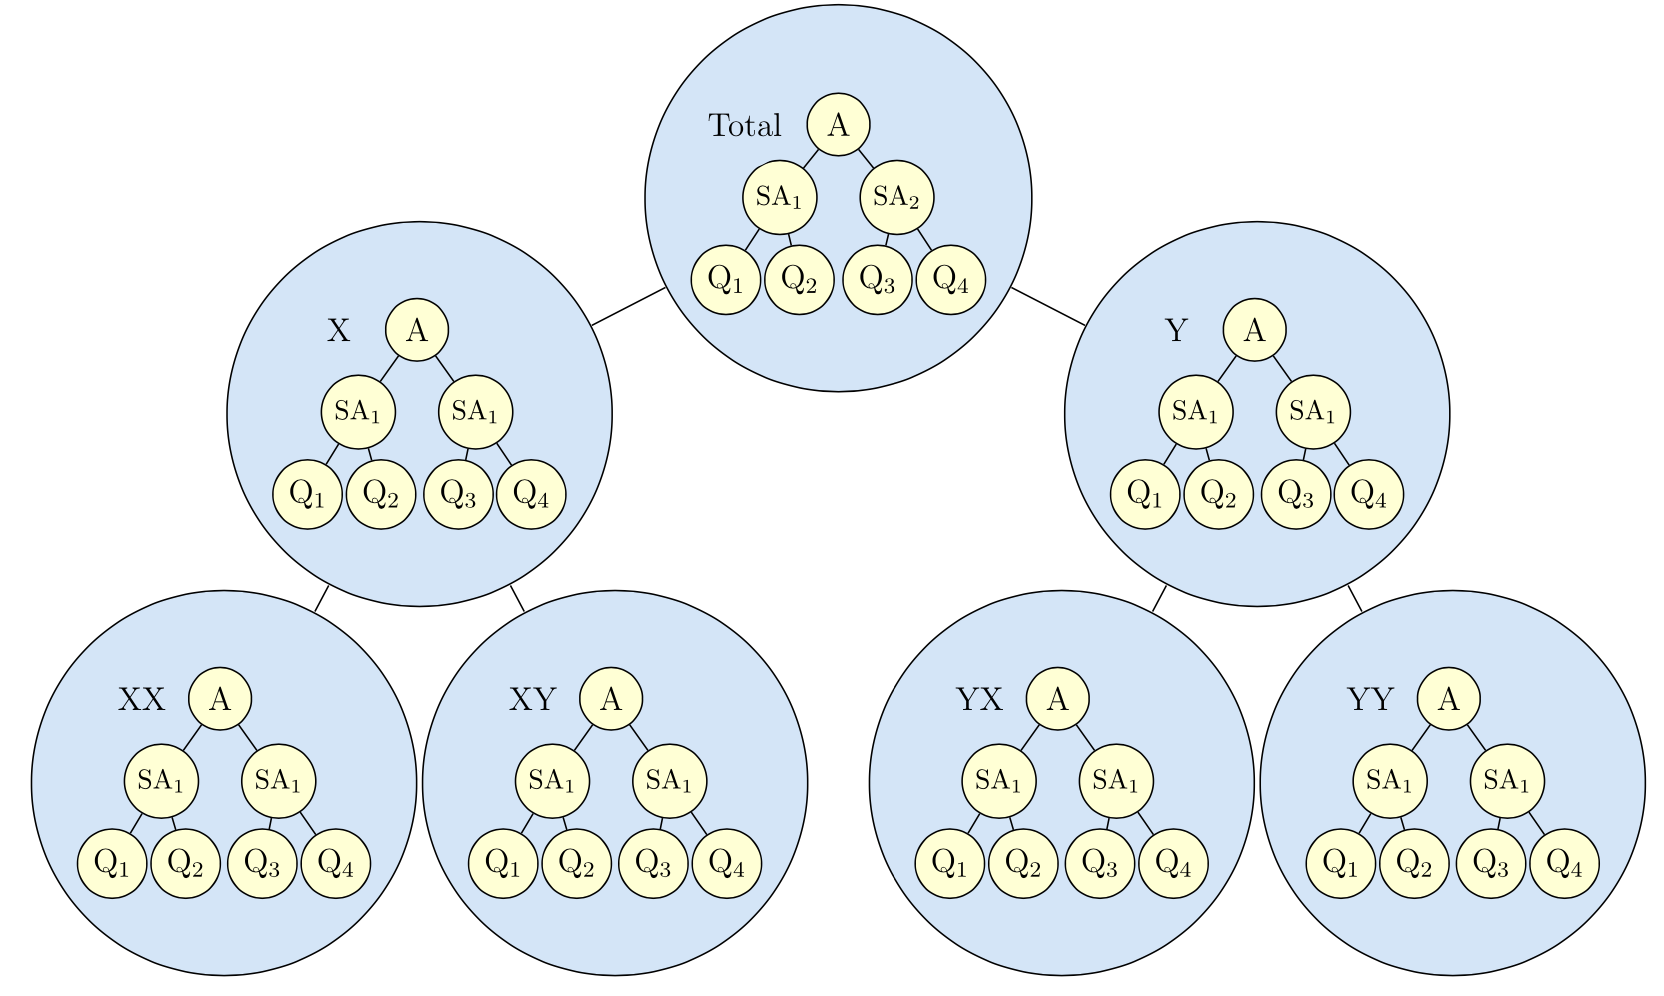
\includegraphics{image/cross-temporal.png}

}

\caption{\label{fig-crosstemp}Cross-temporal hierarchy}

\end{figure}%

\subsection{Forecast reconciliation}\label{forecast-reconciliation}

From the cross-temporal hierarchies, forecasts can be produced at all
levels for every nodes. And in an ideal scenario, forecasts from
different levels of aggregation could seamlessly sum up to the top
level. However, practical implementation often reveals incoherent among
independently produced forecasts. Each independently produced forecast
is subject to different errors, and the summation of these errors from
different nodes results in aggregated forecasts that differ from the
independently produced forecast at the top level. Consequently, it
becomes vital for forecasts to align and aggregate according to the
hierarchical structure organizing the array of time series. As a
solution to this challenge, forecast reconciliation emerges as one of
the most effective methodologies employed to date.

We first consider cross-sectional forecast reconciliation. Recall from
Figure~\ref{fig-crosssec}, we can construct this hierarchical structure
for LTD in a matrix form like this:

\[
\begin{bmatrix}
  \text{Total}_{t} \\
  \text{Non-residential}_{t} \\
  \text{Residential}_{t} \\
  \text{Commercial}_{t} \\
  \text{Industrial}_{t} \\
  \text{Other}_{t} \\
  \end{bmatrix}
=
\begin{bmatrix}
  1 & 1 & 1 & 1 \\
  0 & 1 & 1 & 1 \\
  1 & 0 & 0 & 0 \\
  0 & 1 & 0 & 0 \\
  0 & 0 & 1 & 0 \\
  0 & 0 & 0 & 1 \\
\end{bmatrix}
\begin{bmatrix}
  \text{Residential}_{t} \\
  \text{Commercial}_{t} \\
  \text{Industrial}_{t} \\
  \text{Other}_{t} \\
\end{bmatrix}
\]

or in a more compact notation:

\[
\textbf{y}_{t} = \textbf{S}\textbf{b}_{t},
\]

where \(\textbf{y}_t\) is an \(n\)-dimensional vector of all the
observations in the hierarchy at time \(t\), \(\bf{S}\) represents the
summing matrix defining how bottom-level series are aggregated, and
\(\textbf{b}_t\) is an \(m\)-dimensional vector of all the observations
in the bottom level of the hierarchy at time \(t\). In this case, \(n\)
and \(m\) equal to 6 and 4, respectively.

Then for any set of base forecast, denoted as \(\bf{\hat{y}}_{h}\),
where h is the forecast horizon, all reconciliation forecasting
approaches, generating coherent forecasts \(\bf{\tilde{y}}_{h}\), can be
represented as:

\[
\bf{\tilde{y}}_{h} = \bf{SG}\hat{\bf{y}}_{h},
\] where \(\bf{G}\) is a matrix that maps the base forecasts into the
bottom level (\textcite{hyndman2021forecasting}).

The equation shows that pre-multiplying any set of base forecasts with
\(\bf{SG}\) will return a set of coherent forecasts.

Within the domain of hierarchical time series forecasting, there are
three traditional single level approaches for generating forecasts for
hierarchical time series. The first, known as the \emph{bottom-up}
approach, initiates by producing forecasts for each series at the lowest
level and subsequently aggregates these to generate forecasts for the
upper levels of the hierarchy. For this approach, \(\bf{G}\) can be
defined as:

\[
\textbf{G}
=
\begin{bmatrix}
  0 & 0 & 1 & 0 & 0 & 0 \\
  0 & 0 & 0 & 1 & 0 & 0 \\
  0 & 0 & 0 & 0 & 1 & 0 \\
  0 & 0 & 0 & 0 & 0 & 1 \\
\end{bmatrix},
\] where the first 2 columns zero out the base forecast of the series
above the bottom level.

Conversely, the \emph{top-down} approach starts with a forecast at the
highest level, which is then disaggregated to lower levels using
predetermined proportions---typically based on historical data
distributions (\textcite{gross1990disaggregation}). For this approach,
\(\bf{G}\) can be defined as:

\[
\textbf{G}
=
\begin{bmatrix}
  \text{p}_{1} & 0 & 0 & 0 & 0 & 0 \\
  \text{p}_{2} & 0 & 0 & 0 & 0 & 0 \\
  \text{p}_{3} & 0 & 0 & 0 & 0 & 0 \\
  \text{p}_{4} & 0 & 0 & 0 & 0 & 0 \\
\end{bmatrix},
\] where the first column includes the set of proportions that
distribute the base forecasts of the top level to the bottom level

Lastly, the \emph{middle-out} approach is a combination of both the
bottom-up and top-down methods.

However, the traditional single level approaches may have their
limitations since only base forecast at one level is used. In response
to this, \textcite{wickramasuriya2018optimal} introduced the \emph{MinT}
(Minimum Trace) optimal reconciliation methodology, which is based on
the finding of a \textbf{G} matrix that minimises the total forecast
variance within the set of coherent forecasts.

\textcite{wickramasuriya2018optimal} show that the variance-covariance
of the h-step-ahead coherent forecast errors is given by: \[
\textbf{V}_{h} = Var[\textbf{y}_{T+h} - \bf{\tilde{y}}_\text{h}] = \textbf{SG}\textbf{W}_{h}\textbf{G'S'} ,
\] where \(\textbf{W}_{h} = Var[\textbf{y}_{T+h} - \bf{\hat{y}}_{h}]\)
is the variance-covariance matrix of the corresponding base forecast
errors.

\textcite{wickramasuriya2018optimal} also show that: \[
\textbf{G} = (\textbf{S}'\textbf{W}_{h}^{-1}\textbf{S})^{-1}\textbf{S}'\textbf{W}_{h}^{-1},
\] minimises the trace of \(\textbf{V}_{h}\) subject to \textbf{S}
\textbf{G} \textbf{S} = \textbf{S}

Therefore, the optimally reconciled forecasts are given by: \[
\bf{\tilde{y}}_{h} = \textbf{S}(\textbf{S}'\textbf{W}_{h}^{-1}\textbf{S})^{-1}\textbf{S}'\textbf{W}_{h}^{-1}\bf{\hat{y}}_{h}
\] which refers as the \textbf{MinT}

Now, a challenge with G is that it requires an estimation of
\(\textbf{W}_{h}\), the forecast error variance of h-step-ahead base
forecasts. There are four simplifying approximations in place that have
been shown to work well:

\begin{enumerate}
\def\labelenumi{\arabic{enumi}.}
\tightlist
\item
  \textbf{OLS} (\textcite{hyndman2011optimal}):
  \(\mathbf{W}_{h} = \text{k}_{h}\mathbf{I}\) for all h, where
  \(\text{k}_{h} > 0\).
\end{enumerate}

This is the most simplifying assumption to make, and means that
\(\bf{G}\) is independent of the data, providing substantial
computational savings. The disadvantage, however, is that this
specification does not account for the differences in scale between the
levels of the structure, or for relationships between series.

This is the simplest assumption to adopt, implying that \(\bf{G}\) is
independent of the data, which significantly reduces computational
costs. However, this approach does not account for the varying scales
across different levels of the structure or for the relationships
between series.

\begin{enumerate}
\def\labelenumi{\arabic{enumi}.}
\setcounter{enumi}{1}
\tightlist
\item
  \(\bf{WLS}_{S}\) (\textcite{athanasopoulos2017forecasting}):
  \(\mathbf{W}_{h} = \text{k}_{h}\mathbf{\Lambda}\) for all h, where
  \(\text{k}_{h} > 0\), \(\mathbf{\Lambda} = diag(\textbf{S1})\), and
  \(\bf{1}\) is unit vector of dimension \(\it{m}\) (the number of
  bottom-level series).
\end{enumerate}

Applying structural scaling is particularly useful in cases where
residuals are not available, and so the variance scaling cannot be
applied; for example, in cases where the base forecasts are generated by
judgemental forecasting.

\begin{enumerate}
\def\labelenumi{\arabic{enumi}.}
\setcounter{enumi}{2}
\tightlist
\item
  \(\bf{WLS}_{V}\) (\textcite{hyndman2016fast}):
  \(\mathbf{W}_{h} = \text{k}_{h}\text{diag(}\mathbf{\hat{W}}_{1}\text{)}\)
  for all h, where \(\text{k}_{h} > 0\),
\end{enumerate}

\[
\mathbf{\hat{W}}_{1} = \frac{1}{T}\sum_{t=1}^{T}\textbf{e}_{t}\textbf{e'}_{t},
\] and \(\textbf{e}_{t}\) is an \(\it{n}\)-dimensional vector of
residuals of the models that generated the base forecasts stacked in the
same order as the data.

\begin{enumerate}
\def\labelenumi{\arabic{enumi}.}
\setcounter{enumi}{3}
\tightlist
\item
  \(\bf{MinT}_{S}\) (\textcite{wickramasuriya2018optimal}):
  \(\mathbf{W}_{h} = \text{k}_{h}\mathbf{\hat{W}^{*}}_{1, D}\) for all
  h, where \(\text{k}_{h} > 0\), and
  \(\mathbf{\hat{W}^{*}}_{1, D} = \mathit{\lambda}\mathbf{\hat{W}^{*}}_{1, D} + \text{(1-} \mathit{\lambda})\mathbf{\hat{W}}_{1}\)
  is a shrinkage estimator with diagonal target
  \(\mathbf{\hat{W}^{*}}_{1, D}\), a diagonal matrix comprising the
  diagonal entries of \(\mathbf{\hat{W}}_{1}\), and \(\mathit{\lambda}\)
  the shrinkage intensity parameter.
\end{enumerate}

In contrast to earlier estimators of variance and structural scaling,
this method captures strong interrelationships between time series in
the hierarchy, while the use of shrinkage helps to manage the complexity
of the estimation due to the size of \(\mathbf{W}_{h}\).

By following the above procedure, we will get cross-sectionally coherent
forecasts. Moreover, this procedure extends to temporal reconciliation
and cross-temporal reconciliation.

\subsubsection{Cross-sectional
reconciliation}\label{cross-sectional-reconciliation}

For cross-sectional reconciliation, there are two main challenges, as
stated by \textcite{kourentzes2019cross}:

\begin{enumerate}
\def\labelenumi{\arabic{enumi}.}
\tightlist
\item
  the size of the cross-sectional dimension of the hierarchy; and
\item
  the heterogeneity of the series across, but also within levels.
\end{enumerate}

The size relates directly with estimation of \(\mathbf{W}_{h}\), and
therefore very large hierarchies, estimation of \(\mathbf{W}_{h}\) can
be computationally expensive. However, this is not the case for this
hierarchical structure in Figure~\ref{fig-crosssec}. On the other hand,
it is expected that there will be heterogeneity between each
cross-sectional levels. Therefore, in this case, we choose not to apply
structural scaling since it assumes that each of the bottom-level base
forecasts has errors with equal variance \(\text{k}_{h}\).

\subsubsection{Temporal reconciliation}\label{temporal-reconciliation}

On the other hand, for temporal hierarchies, forecasts across all levels
are for the same series, therefore it is safe to assume homogeneity
between each level. On the other hand, following the arguments by
\textcite{athanasopoulos2017forecasting}, since the covariances in
\(\mathbf{W}_{h}\) would be between series of different sampling
frequencies due to the temporal aggregation, we do not implement the
MinT shrinkage estimator.

\subsubsection{Cross-temporal
reconciliation}\label{cross-temporal-reconciliation}

The cross-temporal reconciliation methodology used in this context is
heuristic first-temporal-then-cross-sectional reconciliation, proposed
by \textcite{kourentzes2019cross}. It is a 2-step approach, where step 1
includes reconciliation through temporal hierarchies for each single
variable to achieve temporally coherence forecast (\textbf{THieFs}).
Then for step 2, from previously \textbf{THieFs}, we generate k
cross-sectional reconciliations, setting
\(\textbf{W}_{h} = \bf{\hat{W}}_{h,\ell}\), where \(\ell = 1,2,..,k\),
and k denotes the number of temporal aggregation levels. This results in
reconciliation matrix \(\textbf{SG}_{\ell}\) for each temporal
aggregation level. And by averaging across these, we compose a consesus
reconciliation matrix \textbf{SG}, where
\(\textbf{G} = \frac{1}{k}\sum_{\ell=1}^{k}\textbf{G}_{\ell}\),
capturing the reconciliation consesus across all \emph{k} temporal
aggregation levels. The outcome are cross-temporally reconciled
forecasts, which are coherent across both dimensions, at all scales.

\subsection{Model Selection}\label{model-selection}

As discussed in Section~\ref{sec-coint}, it highlights the pertinence of
employing VECM to adequately model these relationships.

One limitation of these models is their reliance on ample data to
produce reliable parameters. Monthly data spanning over a decade for LTD
has been found to be sufficient. Nevertheless, the subsequent section on
cross-validation will elaborate on the precise sizing of the training
dataset required to ensure compatibility with the VAR and VECM models.

In addition to VAR and VECM, the Autoregressive Integrated Moving
Average (ARIMA) model has also been employed, primarily for purposes of
comparison and validation of improvements. The efficacy of this
comparison will be assessed through time series cross-validation,
utilizing various accuracy metrics such as:

\begin{itemize}
\tightlist
\item
  \emph{Root Mean Square Error (RMSE)}, where the RMSE is computed as:
\end{itemize}

\(\text{RMSE} = \sqrt{\frac{1}{n} \sum_{t=1}^{n} (y_t - \hat{y}_t)^2}\);
and

\begin{itemize}
\tightlist
\item
  \emph{Mean Absolute Percentage Error (MAPE)}, where the MAPE is
  computed by defining the percentage error, to overcome
  scale-dependency of RMSE as:
\end{itemize}

\(\text{MAPE} = \frac{1}{n} \sum_{t=1}^{n} \left| 100 \times \frac{y_t - \hat{y}_t}{y_t} \right|\).

\section{Time Series
Cross-Validation}\label{time-series-cross-validation}

\subsection{Definition and rationale}\label{definition-and-rationale}

Time series cross-validation represents a sophisticated adaptation of
the conventional training/test set approach for model selection, as
stated by \textcite{hyndman2021forecasting}. This methodology is
particularly well-suited to time series data because it exclusively
includes observations from periods prior to those being forecasted,
distinguishing it from traditional cross-validation techniques.

In the scope of this project, time series cross-validation is employed
to rigorously evaluate whether the VAR/VECM or ARIMA models yield more
accurate forecasts for this dataset across forecasting horizons ranging
from 1 to 12 steps ahead. Additionally, this approach is used to gauge
the extent of improvement introduced by the reconciliation process in
comparison to the base forecasts. Time series cross-validation
facilitates the generation of a series of 1 to 12-step-ahead forecasts
across various rolling periods. For instance, a 12-step-ahead forecast
can be produced starting from January 2022, followed by another
12-step-ahead forecast from February 2022, and so forth. This is
essential for the \emph{Department of Treasury and Finance} to analyze
the effects of market dynamics or policy changes on land transfer duty.

The initial training set will start with 108 monthly observations,
equating to 9 years of data, and will roll forward by 1 month for each
subsequent step. This process will generate 10 folds of training sets,
and thus there will be 10 sets of 12-step-ahead forecasts with
equivalent test set for forecasting accuracy evaluation . While the
number of observations in the initial training set can be lower, 108
months were chosen for code efficiency.

\subsection{Generating forecast}\label{generating-forecast}

To enhance forecast accuracy, this methodology extends beyond a
cross-sectional hierarchical structure to incorporate a temporal
hierarchical structure, culminating in cross-temporal reconciliation
forecasting. This approach integrates forecasts across different time
structures, and its efficacy is evaluated by comparing it with
cross-sectional and temporal reconciliation forecasts individually to
determine any improvements.

Given the monthly frequency of the data, additional aggregation levels
such as bi-monthly, quarterly, four-monthly, semi-annually, and annually
are established, with the annual aggregation representing the top level
of the temporal hierarchy.

Models are fitted at each cross-sectional level across these varying
temporal frequencies. A loop is utilized to generate forecasts and
residuals, which are subsequently organized into a matrix for each
temporal frequency: monthly (denoted as k1), bi-monthly (k2), quarterly
(k3), four-monthly (k4), semi-annually (k6), and annually (k12). These
matrices are then collectively stored within a list.

This structured approach facilitates the fitting of different models
tailored to each temporal frequency, allowing for adjustments in
argument values as necessary. Moreover, if a distinct model is required
for various cross-sectional levels, an \texttt{if} condition is employed
within each temporal frequency loop to ensure this customization. The
forecasts and residuals are then allocated to \texttt{base} and
\texttt{res} data structures, respectively.

\subsubsection{ARIMA}\label{arima}

The ARIMA model will be implemented across all levels of the temporal
hierarchical structure and at every cross-sectional level. Since as
discussed in Section~\ref{sec-tsanalysis}, there is seasonal pattern for
some nodes, such as total land transfer duty, residential property land
transfer duty or sales. And thus we will pay more attention on seasonal
ARIMA model. It is a combination of differencing with autoregression and
a moving average model. The full model can be written as:

\[
y'_t = c + \phi_1 y'_{t-1} + \cdots + \phi_p y'_{t-p} + \Phi_1 y'_{t-m} + \cdots + \Phi_P y'_{t-mP} + \theta_1 \varepsilon_{t-1} + \cdots + \theta_q \varepsilon_{t-q} + \Theta_1 \varepsilon_{t-m} + \cdots + \Theta_Q \varepsilon_{t-mQ} + \varepsilon_t,
\]

where:

\begin{itemize}
\tightlist
\item
  \(y'_t\) is the differenced series, considering both non-seasonal and
  seasonal differencing.
\item
  \(\phi_i\) are the coefficients for the non-seasonal autoregressive
  (AR) terms.
\item
  \(\theta_j\) are the coefficients for the non-seasonal moving average
  (MA) terms.
\item
  \(\Phi_k\) are the coefficients for the seasonal autoregressive (SAR)
  terms.
\item
  \(\Theta_l\) are the coefficients for the seasonal moving average
  (SMA) terms.
\item
  \(\varepsilon_t\) is the white noise error term.
\item
  \(m\) is the seasonal period.
\end{itemize}

The parameters are defined as follows:

\begin{longtable}[]{@{}rl@{}}
\toprule\noalign{}
Parameter & Description \\
\midrule\noalign{}
\endhead
\bottomrule\noalign{}
\endlastfoot
( p ) & order of the non-seasonal autoregressive part; \\
( d ) & degree of non-seasonal differencing involved; \\
( q ) & order of the non-seasonal moving average part; \\
( P ) & order of the seasonal autoregressive part; \\
( D ) & degree of seasonal differencing involved; \\
( Q ) & order of the seasonal moving average part; \\
( m ) & number of periods in each season. \\
\end{longtable}

Or it can be written as:

\[
\text{ARIMA} \quad 
\begin{array}{c}
(p, d, q) \quad (P, D, Q)_m \\
\underbrace{\phantom{(p, d, q)}} \quad \underbrace{\phantom{(P, D, Q)_m}} \\
\text{Non-seasonal part} \quad \text{Seasonal part} \\
\text{of the model} \quad \text{of the model}
\end{array},
\] where \(m\) is the seasonal period (e.g., number of observations per
year)

To implement this, we can use the \texttt{auto.arima()} function from
the \texttt{forecast} package. This function efficiently determines the
optimal parameters for the autoregressive lag, differencing, and moving
average components of the model by automatically adjusting them for the
error terms.

\subsubsection{VAR/VECM}\label{varvecm}

A vector autoregression model of order 1, VAR(1) between 2 time series
can be represented with:

\[
\begin{aligned}
y_t &= \beta_{10} + \beta_{11} y_{t-1} + \beta_{12} x_{t-1} + \nu_t^y \\
x_t &= \beta_{20} + \beta_{21} y_{t-1} + \beta_{22} x_{t-1} + \nu_t^x
\end{aligned}
\] Then the one-step-ahead forecasts are generated by:

\[
\begin{aligned}
\hat{y}_{T+1|T} &= \hat{\beta}_{10} + \hat{\beta}_{11} y_{T} + \hat{\beta}_{12} x_{T} \\
\hat{x}_{T+1|T} &= \hat{\beta}_{20} + \hat{\beta}_{21} y_{T} + \hat{\beta}_{22} x_{T}
\end{aligned}
\]

The VAR(1) equation can be extended to lag of 3 between 3 time series,
which is our case:

\[
\begin{aligned}
y_t &= \beta_{10} + \beta_{11} y_{t-1} + \beta_{12} x_{t-1} + \beta_{13} z_{t-1} + \beta_{14} y_{t-2} + \beta_{15} x_{t-2} + \beta_{16} z_{t-2} + \beta_{17} y_{t-3} + \beta_{18} x_{t-3} + \beta_{19} z_{t-3} + \nu_t^y \\
x_t &= \beta_{20} + \beta_{21} y_{t-1} + \beta_{22} x_{t-1} + \beta_{23} z_{t-1} + \beta_{24} y_{t-2} + \beta_{25} x_{t-2} + \beta_{26} z_{t-2} + \beta_{27} y_{t-3} + \beta_{28} x_{t-3} + \beta_{29} z_{t-3} + \nu_t^x \\
z_t &= \beta_{30} + \beta_{31} y_{t-1} + \beta_{32} x_{t-1} + \beta_{33} z_{t-1} + \beta_{34} y_{t-2} + \beta_{35} x_{t-2} + \beta_{36} z_{t-2} + \beta_{37} y_{t-3} + \beta_{38} x_{t-3} + \beta_{39} z_{t-3} + \nu_t^z
\end{aligned},
\] where \(y_t\), \(x_t\) and \(z_t\) represent land transfer duty,
sales and home value index.

However, as discussed in Section~\ref{sec-coint}, given the existence of
at least two cointegration relationships among the three time series,
which are different type of property land transfer duty against sales
and home value index, fitting a VECM is more appropriate. The VECM is
formulated by incorporating the error correction term into the VAR model
in first differences. For the three time series ( y\_t ), ( x\_t ), and
( z\_t ), the VECM(3) can be expressed as:

\[
\begin{aligned}
\Delta y_t &= \alpha_1 (\gamma_{11} y_{t-1} + \gamma_{12} x_{t-1} + \gamma_{13} z_{t-1} - \mu_1) + \sum_{j=1}^{3} \left( \beta_{1j1} \Delta y_{t-j} + \beta_{1j2} \Delta x_{t-j} + \beta_{1j3} \Delta z_{t-j} \right) + \varepsilon_t^y \\
\Delta x_t &= \alpha_2 (\gamma_{21} y_{t-1} + \gamma_{22} x_{t-1} + \gamma_{23} z_{t-1} - \mu_2) + \sum_{j=1}^{3} \left( \beta_{2j1} \Delta y_{t-j} + \beta_{2j2} \Delta x_{t-j} + \beta_{2j3} \Delta z_{t-j} \right) + \varepsilon_t^x \\
\Delta z_t &= \alpha_3 (\gamma_{31} y_{t-1} + \gamma_{32} x_{t-1} + \gamma_{33} z_{t-1} - \mu_3) + \sum_{j=1}^{3} \left( \beta_{3j1} \Delta y_{t-j} + \beta_{3j2} \Delta x_{t-j} + \beta_{3j3} \Delta z_{t-j} \right) + \varepsilon_t^z
\end{aligned}
\]

where:

\begin{itemize}
\tightlist
\item
  \(\Delta y_t\), \(\Delta x_t\), and \(\Delta z_t\) represent the first
  differences of \(y_t\), \(x_t\), and \(z_t\), respectively.
\item
  \(\alpha_i\) are the adjustment coefficients for the error correction
  terms.
\item
  \(\gamma_{ij}\) are the coefficients of the cointegrating vectors.
\item
  \(\mu_i\) are the constants in the cointegration relationships.
\item
  \(\varepsilon_t^y\), \(\varepsilon_t^x\), and \(\varepsilon_t^z\) are
  the white noise error terms.
\end{itemize}

The VECM framework thus captures both the short-term dynamics through
the differenced terms and the long-term equilibrium relationships
through the error correction terms.

Finally, the reconciliation procedure can be implemented using the
\texttt{FoReco} package \textcite{FoReco}.

\section{Results}\label{results}

\subsection{RMSE}\label{rmse}

\begin{figure}

\centering{

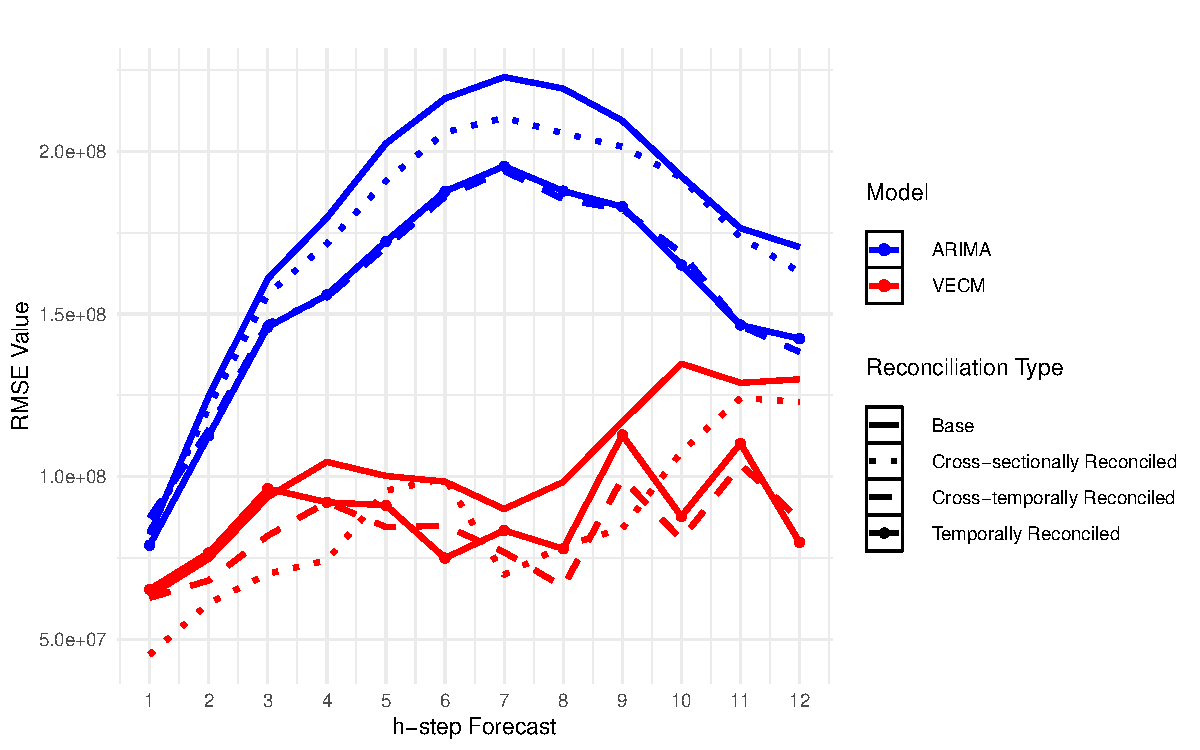
\includegraphics{Report_files/figure-pdf/fig-rmse-1.pdf}

}

\caption{\label{fig-rmse}Monthly total LTD base and reconciled forecast
RMSE by model}

\end{figure}%

Figure~\ref{fig-rmse} illustrates the Root Mean Square Error (RMSE) of
reconciled forecasts in comparison to base forecasts for both VECM and
ARIMA models. The blue lines denote the ARIMA model, while the red lines
represent the VECM. The line types are differentiated as follows: solid
lines for base forecasts, solid lines with circle markers for temporally
reconciled forecasts, dotted lines for cross-sectionally reconciled
forecasts, and dashed lines for cross-temporally reconciled forecasts.

Upon initial examination, it is evident that the VECM model consistently
produces more accurate forecasts compared to the ARIMA model, aligning
with the model selection by the \emph{Department of Treasury and
Finance}. Furthermore, the significant disparity between reconciled
forecasts and base forecasts, particularly from the four-step-ahead
forecasts onwards for both models, suggests that forecast reconciliation
markedly enhances forecast accuracy. Notably, for both models, the RMSE
lines of temporally reconciled forecasts are closer to those of
cross-temporally reconciled forecasts, compared to the RMSE lines of
cross-sectionally reconciled forecasts. This indicates that temporal
hierarchies play a more substantial role in improving forecast accuracy
compared to cross-sectional hierarchies.

It is also noteworthy that for one to three-step-ahead forecasts, the
base forecasts already exhibit high performance, hence the improvements
from applying forecast reconciliation are not evident.

\subsection{MAPE}\label{mape}

Using the Mean Absolute Percentage Error (MAPE), we anticipate results
consistent with those obtained from the Root Mean Square Error (RMSE),
which is indeed the case as demonstrated in Figure
Figure~\ref{fig-mape}.

\begin{figure}

\centering{

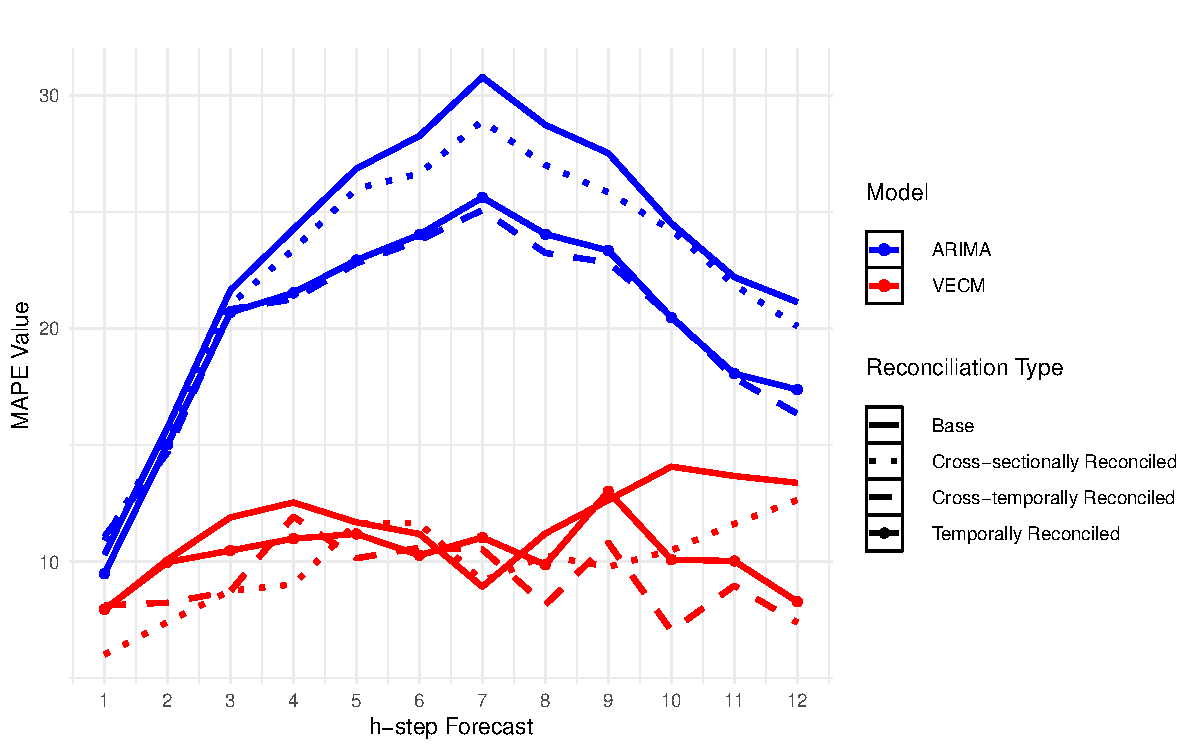
\includegraphics{Report_files/figure-pdf/fig-mape-1.pdf}

}

\caption{\label{fig-mape}Monthly total LTD base and reconciled forecast
MAPE by Method}

\end{figure}%

In conclusion, four key insights can be derived from
Figure~\ref{fig-rmse} and Figure~\ref{fig-mape}:

\begin{enumerate}
\def\labelenumi{\arabic{enumi}.}
\tightlist
\item
  The VECM model is more suitable than the ARIMA model.
\item
  Forecast reconciliation significantly enhances forecast accuracy, with
  cross-temporally reconciled forecasts exhibiting the best performance.
\item
  The majority of the improvement is attributable to incorporating
  temporal hierarchies.
\item
  Forecast reconciliation is particularly effective in improving
  forecasts that initially perform poorly.
\end{enumerate}

\subsection{Comparing against DTF
forecast}\label{comparing-against-dtf-forecast}

The Root Mean Squared Errors (RMSE) of the \emph{Department of Treasury
and Finance} (DTF) forecast were computed utilizing the same time-series
cross-validation procedure as previously described, with the original
scale of land transfer duty serving as a benchmark. As shown in
Figure~\ref{fig-dtfrmse}, the RMSE varies between 110 million and 130
million, with a significant reduction observed at the 12-step-ahead
forecasts. This reduction may be attributed to a strong seasonal pattern
at step 12, which is overlooked when using the original scale of land
transfer duty. Overall, the RMSE derived from the DTF forecast is not
superior to the RMSE of the reconciled forecasts.

\begin{figure}

\centering{

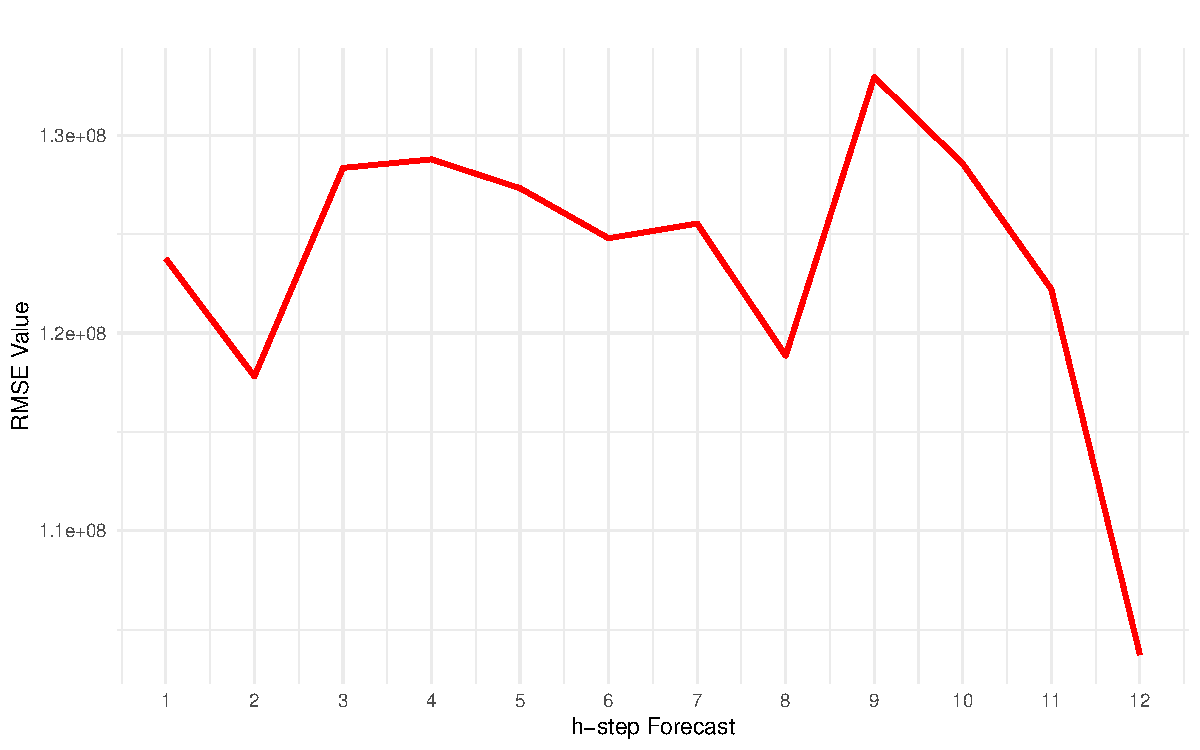
\includegraphics{Report_files/figure-pdf/fig-dtfrmse-1.pdf}

}

\caption{\label{fig-dtfrmse}RMSE of DTF forecast}

\end{figure}%

When extending the comparison to cross-temporally reconciled forecasts
against DTF forecasts, as illustrated in Figure~\ref{fig-rmseratio},
where the red line represents the ratio of MAPE of reconciled forecasts
to DTF forecasts, it is evident that cross-temporally reconciled
forecasts perform significantly better.

\begin{figure}

\centering{

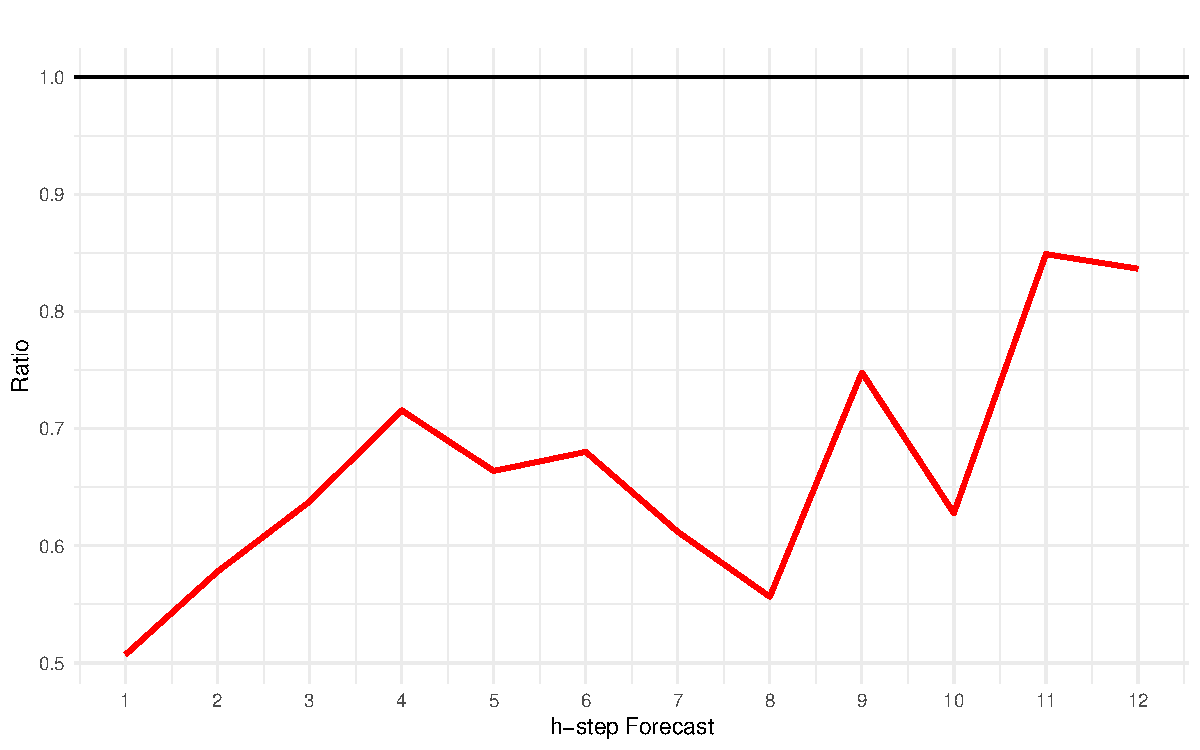
\includegraphics{Report_files/figure-pdf/fig-rmseratio-1.pdf}

}

\caption{\label{fig-rmseratio}Ratio of RMSE of cross-temporally
reconciled forecast to DTF forecast}

\end{figure}%

\section{Discussion}\label{discussion}

\subsection{Interpretation of Results}\label{interpretation-of-results}

The empirical analysis reveals that the VECM model provides more
accurate forecasts for LTD compared to the ARIMA model, particularly
when forecast reconciliation techniques are applied. The incorporation
of cross-sectional and temporal hierarchies into a unified
cross-temporal reconciliation framework markedly improves forecast
accuracy. This indicates that the proposed methodology effectively
captures both short-term dynamics and long-term trends in the property
market.

Temporal reconciliation emerges as more impactful than cross-sectional
reconciliation in enhancing forecast accuracy, underscoring the
importance of temporal aggregation in the forecasting process.

The comparative analysis with the DTF's forecasts further validates the
proposed methodology, demonstrating that cross-temporally reconciled
forecasts consistently outperform the DTF's forecasts, as evidenced by
lower RMSE values.

\subsection{Limitations}\label{limitations}

\begin{itemize}
\item
  \textbf{Seasonal Adjustment}: Although there is a discernible seasonal
  pattern in land transfer duty (LTD), residential LTD
  (\texttt{ltd\_res}), and sales, we did not apply seasonal adjustments.
  Ignoring seasonal adjustments might have affected the model's ability
  to accurately capture seasonal variations, potentially impacting the
  forecast accuracy. Future research could incorporate seasonal
  adjustment methods to address this limitation.
\item
  \textbf{Non-Stationarity in Cointegration Analysis}: When fitting the
  VECM with sales and Home Value Index (HVI) to LTD for non-residential,
  commercial, industrial, and other property types, the Augmented
  Dickey-Fuller (ADF) test on the linear combination of these series,
  based on the eigenvalues from the Johansen test, indicated
  non-stationarity. Non-stationary time series can lead to unreliable
  model estimates and forecasts. To improve stationarity, alternative
  variables could be explored to replace sales and HVI.
\item
  \textbf{Lag Selection for Johansen Test}: The lag length for the
  Johansen test during the 10-fold cross-validation was selected via a
  manual trial-and-error procedure, aiming to achieve the lowest RMSE.
  This manual approach may not identify the optimal lag length
  consistently. Future improvements could involve using cross-validation
  or other automated procedures to systematically determine the optimal
  lag length, enhancing the robustness and reliability of the model
  selection process.
\end{itemize}

\section{Conclusion and
Recommendations}\label{conclusion-and-recommendations}

This study introduced an advanced forecasting methodology for land
transfer duty (LTD) in Victoria, leveraging Vector Error Correction
Model (VECM) and Autoregressive Integrated Moving Average (ARIMA)
models, enhanced by cross-sectional, temporal, and cross-temporal
hierarchies. The findings underscore the superiority of VECM, especially
when coupled with forecast reconciliation techniques, in producing more
accurate forecasts compared to ARIMA. Temporal hierarchies were found to
be more influential than cross-sectional hierarchies in improving
forecast accuracy. The reconciled forecasts consistently outperformed
those of the \emph{Department of Treasury and Finance}, as evidenced by
lower RMSE values. Despite some limitations, such as the lack of
seasonal adjustment and manual lag selection for the Johansen test, the
methodology demonstrates significant potential for enhancing LTD
forecasting accuracy. Future work should focus on addressing these
limitations to further refine the approach and improve its
applicability.

\section{GitHub repo}\label{github-repo}

Here is the \href{https://github.com/justin-git01/ltd_forecasting}{link}
to the GitHub repo of this project.


\printbibliography


\end{document}
